\documentclass[9pt,pdf,utf8,hyperref={unicode},aspectratio=169]{beamer}

%Привычный шрифт для математических формул
\usefonttheme[onlymath]{serif}
\mode<presentation>
{
    \usetheme{boxes}
    \beamertemplatenavigationsymbolsempty

    \setbeamercovered{transparent}
    \setbeamertemplate{navigation symbols}{}
    
    \setbeamertemplate{footline}[frame number]
    \setbeamertemplate{caption}[numbered]
    % \setbeamersize{text margin left=0.5em, text margin right=0.5em}
}

% Дополнительные библиотеки
\usepackage[T2A]{fontenc}
\usepackage[english, russian]{babel}
\usepackage[utf8]{inputenc}
\usepackage{amsmath,amssymb}
\usepackage{indentfirst}
\usepackage{changepage}
\usepackage{enumerate}
\usepackage{mathtools}
\usepackage{multicol}
\usepackage{multirow}
\usepackage{ragged2e}
\usepackage{multicol}
\usepackage{diagbox}
\usepackage{wrapfig}
\usepackage{comment}
\usepackage{subfig}
\usepackage{array}
\usepackage{color}
\usepackage{tikz}
\usepackage{url}
\usepackage{bm}

\usetikzlibrary{trees}

% Определение дополнительных функций
\DeclareMathOperator*{\plim}{\mathop{plim}}
\DeclareMathOperator{\prob}{\mathbf{P}\!}
\DeclareMathOperator{\arctanh}{arctanh}
\DeclareMathOperator{\mmode}{mode}
\DeclareMathOperator{\rank}{rank}
\DeclareMathOperator{\diag}{diag}
\DeclareMathOperator{\sign}{sign}
\DeclareMathOperator{\cov}{cov}
\DeclareMathOperator{\pow}{pow}
\DeclareMathOperator{\med}{med}

\def\argmin#1{ \mathop{\text{argmin}}\limits_{#1} }
\def\argmax#1{ \mathop{\text{argmax}}\limits_{#1} }

\renewcommand{\leq}{\leqslant}
\renewcommand{\geq}{\geqslant}

\DeclareMathOperator{\FWER}{FWER}
\DeclareMathOperator{\FDR}{FDR}
\newtheorem{Th}{Теорема}
\newtheorem{Def}{Определение}

% Основная часть

\title[Анализ зависимостей]{Прикладной статистический анализ данных\\~\\~\\\small{Анализ зависимостей}}
\author{Андрей Грабовой}
\date{}

\begin{document}
\tikzstyle{every node}=[draw=black,thick,anchor=west]
\tikzstyle{selected}=[draw=red,fill=red!30]
\tikzstyle{optional}=[dashed,fill=gray!50]

\begin{frame}
    \titlepage
\end{frame}

\begin{frame}{Задача исследования взаимосвязи между признаками}
%%%%%%%%%%%%%%%%%%%%%%%%%%%%%%%%%%%%%%%%%%%%%%%%%%%%%%%%%%%%%%%%%%%%%%%
% 
%%%%%%%%%%%%%%%%%%%%%%%%%%%%%%%%%%%%%%%%%%%%%%%%%%%%%%%%%%%%%%%%%%%%%%%
	Дано: значения признаков $X_1,X_2$ измерены на объектах $1,\ldots,n.$
	
	Эквивалентная формулировка: имеются связанные выборки $X_1^n = \left(X_{11},\ldots,X_{1n}\right)$ и $X_2^n = \left(X_{21},\ldots,X_{2n}\right)$.
	
	\bigskip
	
	Насколько сильно признаки $X_1,X_2$ связаны между собой?
	
	\bigskip
	
	Статистическая взаимосвязь между случайными величинами~--- \textbf{корреляция}.
\end{frame}

\begin{frame}{Корреляция и причинность}
%%%%%%%%%%%%%%%%%%%%%%%%%%%%%%%%%%%%%%%%%%%%%%%%%%%%%%%%%%%%%%%%%%%%%%%
% В учебниках по статистике можно наи?ти большое количество веселых примеров ложных корреляции?, объясняющихся воздеи?ствием третьего скрытого признака. Например, количество самоубии?ств и радиоприемников на душу населения высоко положительно коррелировано, и это объясняется воздеи?ствием признака «размер города». Уровень углекислого газа в атмосфере планеты и распространенность ожирения также высоко положительно коррелированы — это объясняется ростом со временем уровня жизни. Рыночная доля браузера Internet Explorer и количество убии?ств в США тоже положительно коррелированы, и это объясняется в первую очередь фактором времени: во времени снижается и тот, и другои? показатель.
% Иногда корреляцию между парои? признаков нельзя объяснить даже влиянием никакого третьего другого, а эта корреляция просто случаи?на. Если взять достаточное количество величин и искать среди них все возможные попарные корреляции, наи?де?тся очень много странного. Например, можно показать, что значима положительная корреляция между количеством людеи?, которые утонули при падении в бассеи?н, и количеством фильмов, в которых снялся за год Николас Кеи?дж. Корреляция Пирсона между этими двумя признаками rX1X2 = 0.67. Достигаемыи? уровень значимости критерия Стьюдента: p = 0.0253. 95\% доверительныи? интервал для корреляции Пирсона: [0.110, 0.905]. Несмотря на то, что он довольно широкии?, 0 в не?м не содержится. Тем не менее, абсолютно очевидно, что связать эти два признака какои? бы то ни было цепочкои? причинно-следственных связеи? не представляется возможным. Этот эффект явно случаи?ныи?, и то, что его нашли, — это следствие того, что его очень хорошо искали.
% Главныи? вывод: из корреляции никогда не следует причинно-следственная связь, но из причинно-следственнои? связи часто следуют корреляции. Причинно-следственная связь оставляет в данных какие-то следы, которые можно обнаружить в том числе и корреляционными методами. Однако для этого есть другие специальные методы, связанные с построением графов причинности, и лучше использовать именно их.
%%%%%%%%%%%%%%%%%%%%%%%%%%%%%%%%%%%%%%%%%%%%%%%%%%%%%%%%%%%%%%%%%%%%%%%
		\begin{center}
			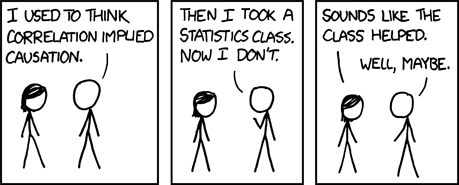
\includegraphics[width=0.3\textwidth]{xkcd.png}
		\end{center}
		\textbf{Корреляция}~--- статистическая взаимосвязь между случайными величинами; не является достаточным условием причинно"=следственной:
		\begin{center}
			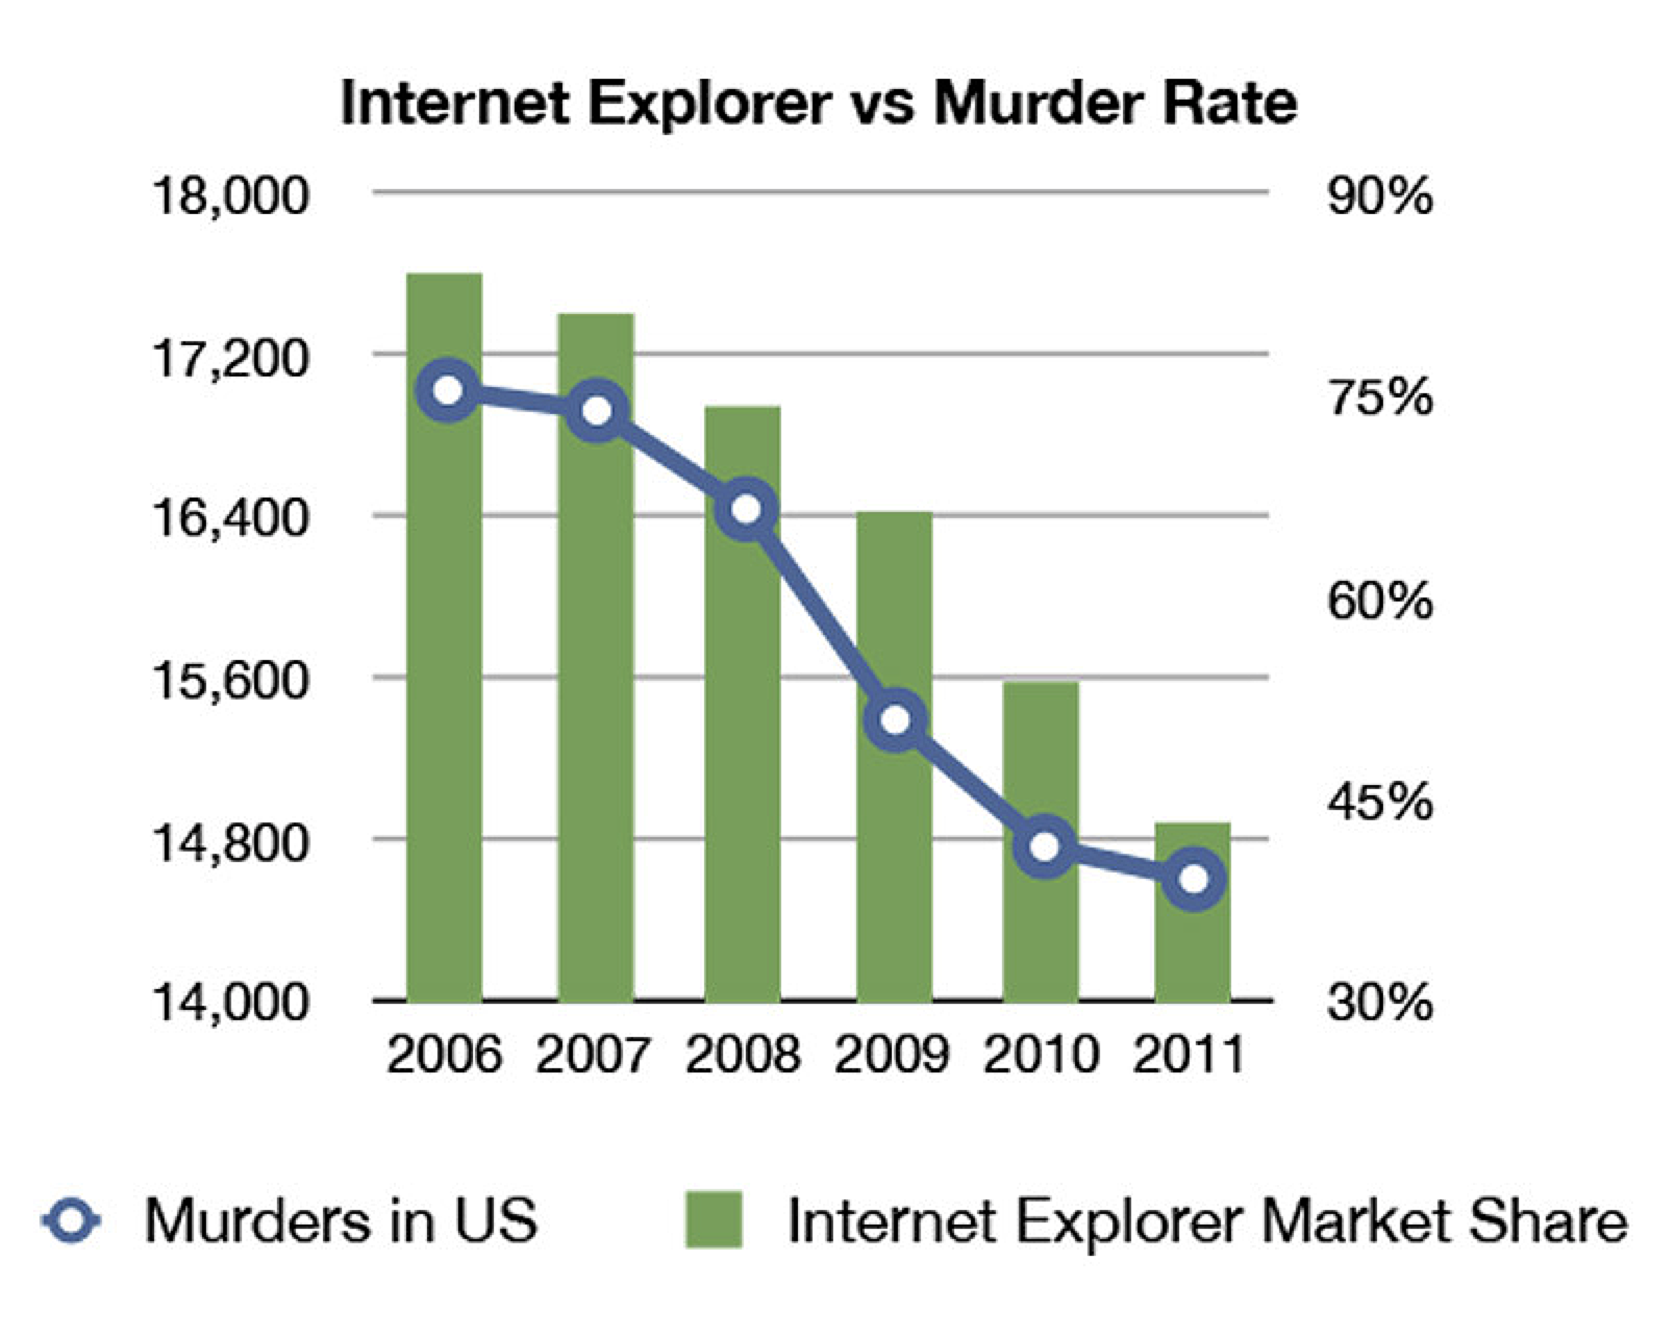
\includegraphics[width=0.35\textwidth]{ievsmurder.png}
		\end{center}
		Другие примеры: \url{http://www.tylervigen.com/}
\end{frame}


\section{Непрерывные признаки}
\subsection{r Пирсона}
\begin{frame}{Корреляция Пирсона}
	\only<1>{
		\textbf{Коэффициент корреляции Пирсона} $r_{X_1X_2}$ случайных величин $X_1$ и $X_2$~--- мера силы \textbf{линейной} корреляции между ними:
		$$r_{X_1X_2} = \frac{\mathbb{E}\left(\left(X_1-\mathbb{E}X_1\right)\left(X_2-\mathbb{E}X_2\right)\right)}{\sqrt{\mathbb{D}X_1\mathbb{D}X_2}}.$$
		
		$r_{X_1X_2}\in\left[-1,1\right]$.
		
		\bigskip
		
		Пусть имеется простая выборка пар $\left(X_{1i},X_{2i}\right), i=1,\dots,n.$
		
		Выборочный коэффициент корреляции Пирсона:
		$$\hat{r}_{X_1X_2} = \frac{ \sum\limits_{i=1}^n \left(X_{1i}-\bar{X}_1\right) \left(X_{2i}-\bar{X}_2\right) }{ \sqrt{\sum\limits_{i=1}^n \left(X_{1i}-\bar{X}_1\right)^2 \sum\limits_{i=1}^n \left(X_{2i}-\bar{X}_2\right)^2 } }.$$
	}
	
	\only<2>{
%%%%%%%%%%%%%%%%%%%%%%%%%%%%%%%%%%%%%%%%%%%%%%%%%%%%%%%%%%%%%%%%%%%%%%%
% На рисунке показаны диаграммы рассеяния — графики, на однои? оси которых отложены значения X1, а на другои? — X2. Первыи? ряд показывает облако точек с идеальнои? положительнои? корреляциеи? (rX1 X2 = 1). Если начать это облако размывать, то коэффициент корреляции Пирсона постепенно уменьшится до 0. Если затем облако точек начать сжимать в обратном направлении, коэффициент растет по модулю и постепенно становится равным ?1. Следующии? эксперимент во втором ряду показывает облако с высокои? положительнои? корреляциеи? между случаи?ными величинами. Если начать его постепенно загибать, то коэффициент корреляции Пирсона будет уменьшаться. Когда форма облака становится похожеи? на параболу, значение выборочного коэффициента корреляции приближается к 0. Так происходит, потому что корреляция Пирсона — это мера силы линеи?нои? взаимосвязи между случаи?ными величинами. То есть все нелинеи?ные функциональные зависимости, даже если они очень хорошо выражены, коэффициент корреляции Пирсона не обнаруживают. Это демонстрируют примеры в третьем ряду. Если между случаи?ными величинами X1 и X2 наблюдаются сложные зависимости, далекие от линеи?ных, коэффициент корреляции Пирсона будет все? равно близким к 0.
% Следующии? важныи? пример изображе?н в нижнем ряду: показано облако из тысячи точек с сильнои? отрицательнои? корреляциеи?. Если взять 5 точек из этого облака и начать постепенно отодвигать в верхнии? правыи? угол диаграммы рассеяния, то, чем дальше отодвигаются эти 5 точек, тем меньше по модулю становится значение выборочного коэффициента корреляции. С какого-то момента оно переходит через 0 и начинает расти. Достаточно сильно отодвинув всего 5 точек из тысячи, можно получить большои? положительныи? коэффициент корреляции. Это говорит о том, что коэффициент корреляции Пирсона неустои?чив к выбросам: небольшое количество точек могут оказывать на него существенное влияние, если они находятся достаточно далеко от основного облака. Это существенная особенность корреляции Пирсона, которую нужно иметь в виду.
%%%%%%%%%%%%%%%%%%%%%%%%%%%%%%%%%%%%%%%%%%%%%%%%%%%%%%%%%%%%%%%%%%%%%%%

		\begin{center}
			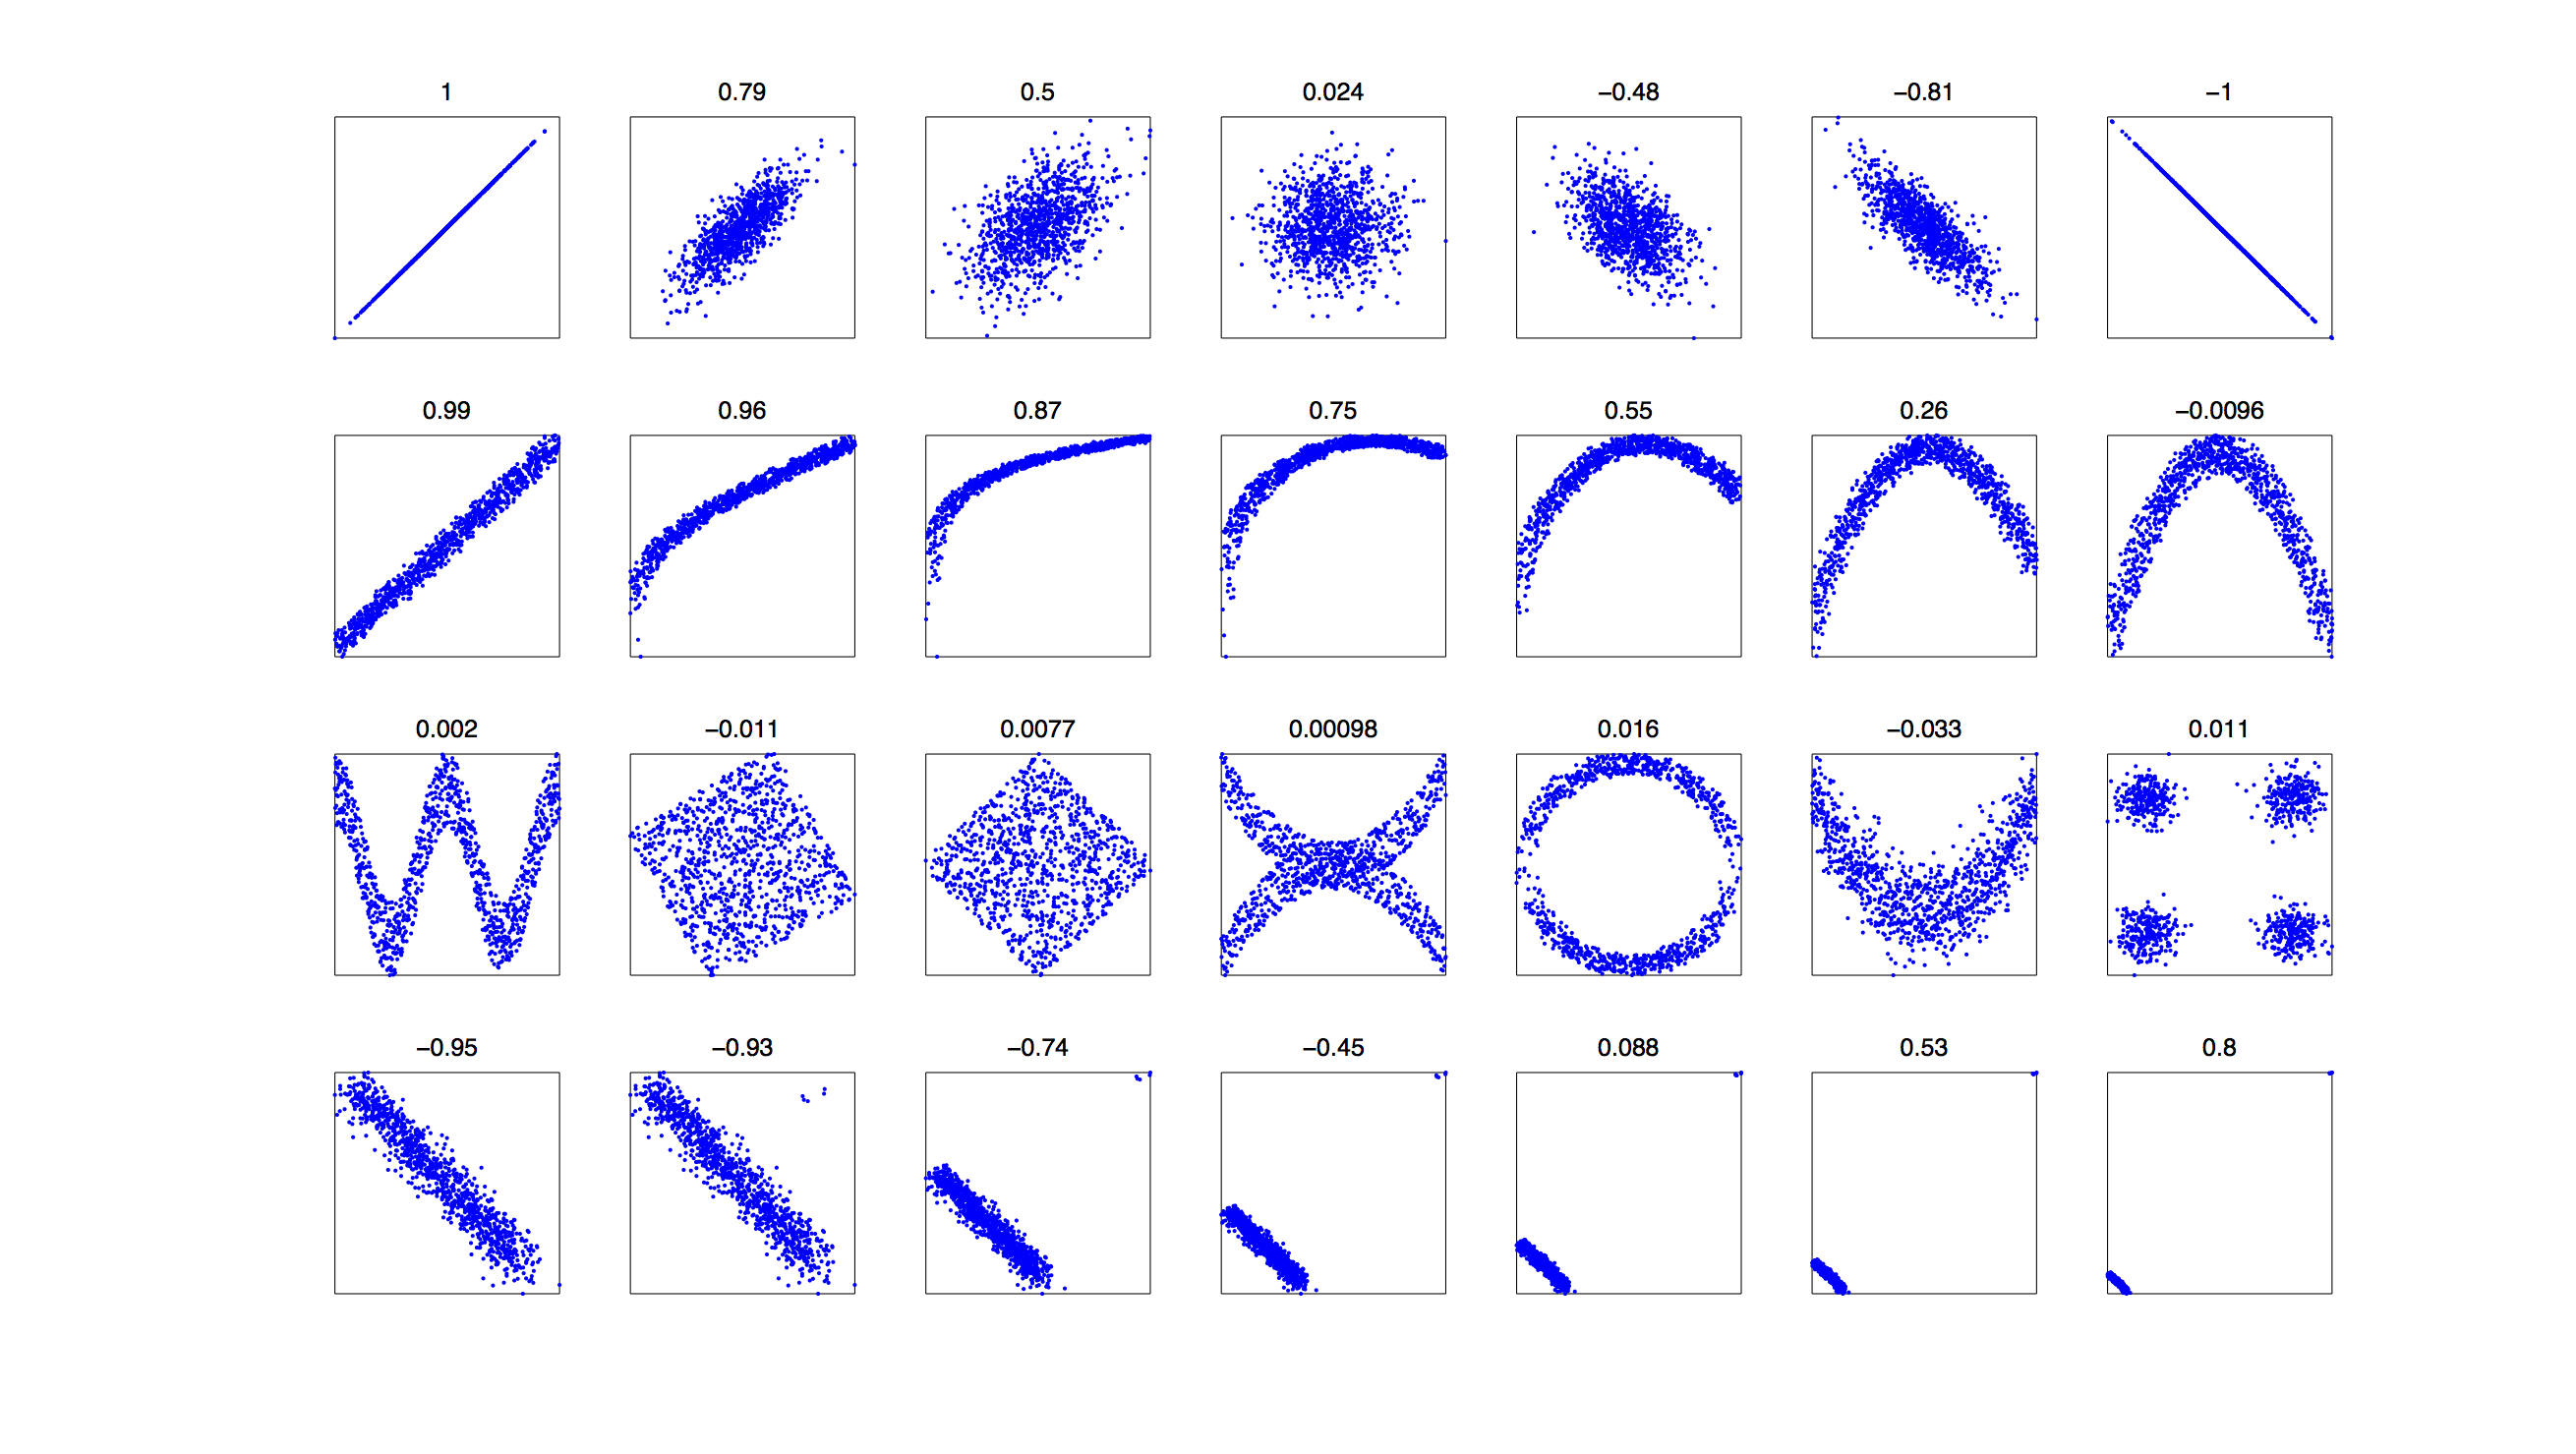
\includegraphics[width=0.8\textwidth,trim=55mm 25mm 40mm 10mm,clip]{corr_pearson.png}
		\end{center}
		\url{http://guessthecorrelation.com/}
	}
	
	\only<3>{
		Недостатки выборочного коэффициента Пирсона:
		\begin{itemize}
			\item для распределений, отличных от нормального, перестаёт быть эффективной оценкой популяционного коэффициента корреляции;
			\item служит мерой только линейной взаимосвязи;
			\item неустойчив к выбросам.
		\end{itemize}
		
		\begin{center}
			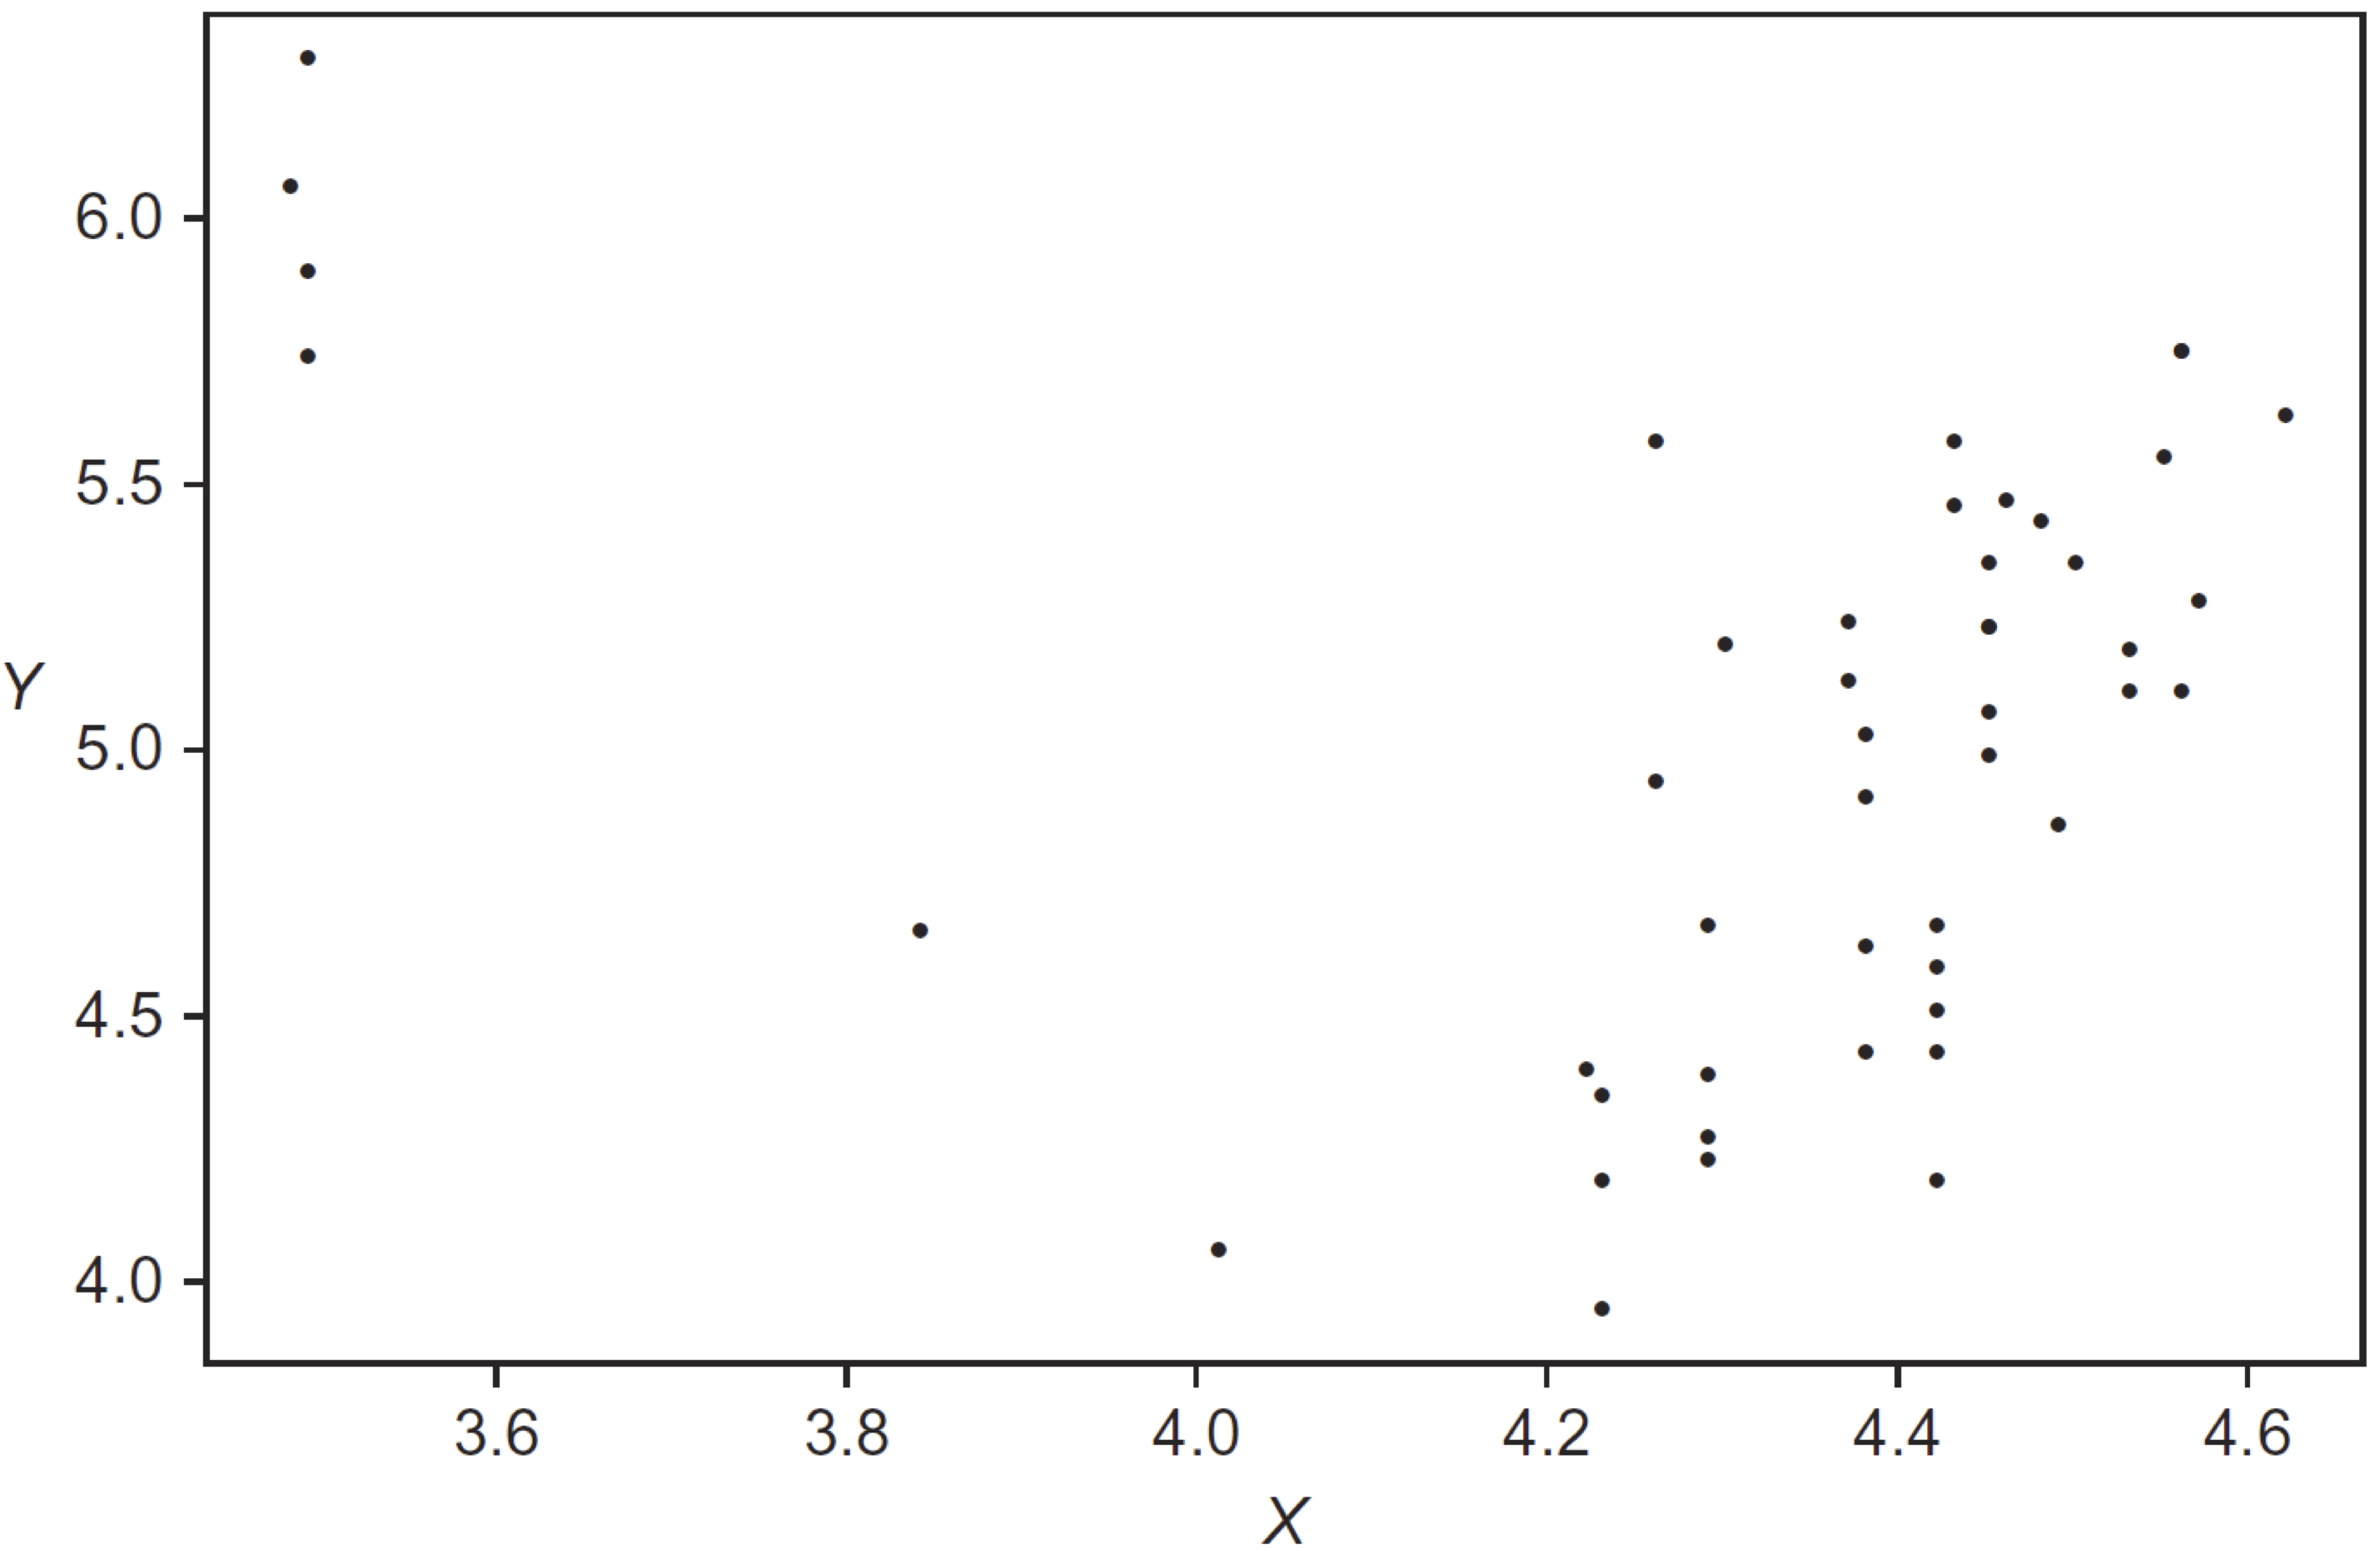
\includegraphics[width=0.45\textwidth]{stars.png}
		\end{center}
		Корреляция между логарифмами эффективной температуры на поверхности звезды ($X$) и интенсивности её света ($Y$) получается отрицательной ($\hat{r}_{XY}=-0.21$) из-за наличия в выборке красных гигантов.    	
	}
\end{frame}

\begin{frame}{Критерий Стьюдента}

		\begin{center}
			\begin{tabular}{rl}
				выборки:                        & $X_1^n=\left(X_{11},\ldots,X_{1n}\right)$\\
				                                & $X_2^n=\left(X_{21},\ldots,X_{2n}\right)$\\
				                                & выборки связанные\\
				                                & $\left(X_{1},X_{2}\right)\sim N\left(\mu,\Sigma\right)$ \\
				нулевая гипотеза:               & $H_0\colon r_{X_1X_2}=0$ \\
				альтернатива:                   & $H_1\colon r_{X_1X_2}<\neq>0$ \\
				статистика:                     & $T\left(X_1^n, X_2^n\right) = \frac{\hat{r}_{X_1X_2} \sqrt{n-2}}{\sqrt{1-\hat{r}^2_{X_1X_2}}}$ \\
				нулевое распределение:          & $St(n-2)$\\
			\end{tabular}
			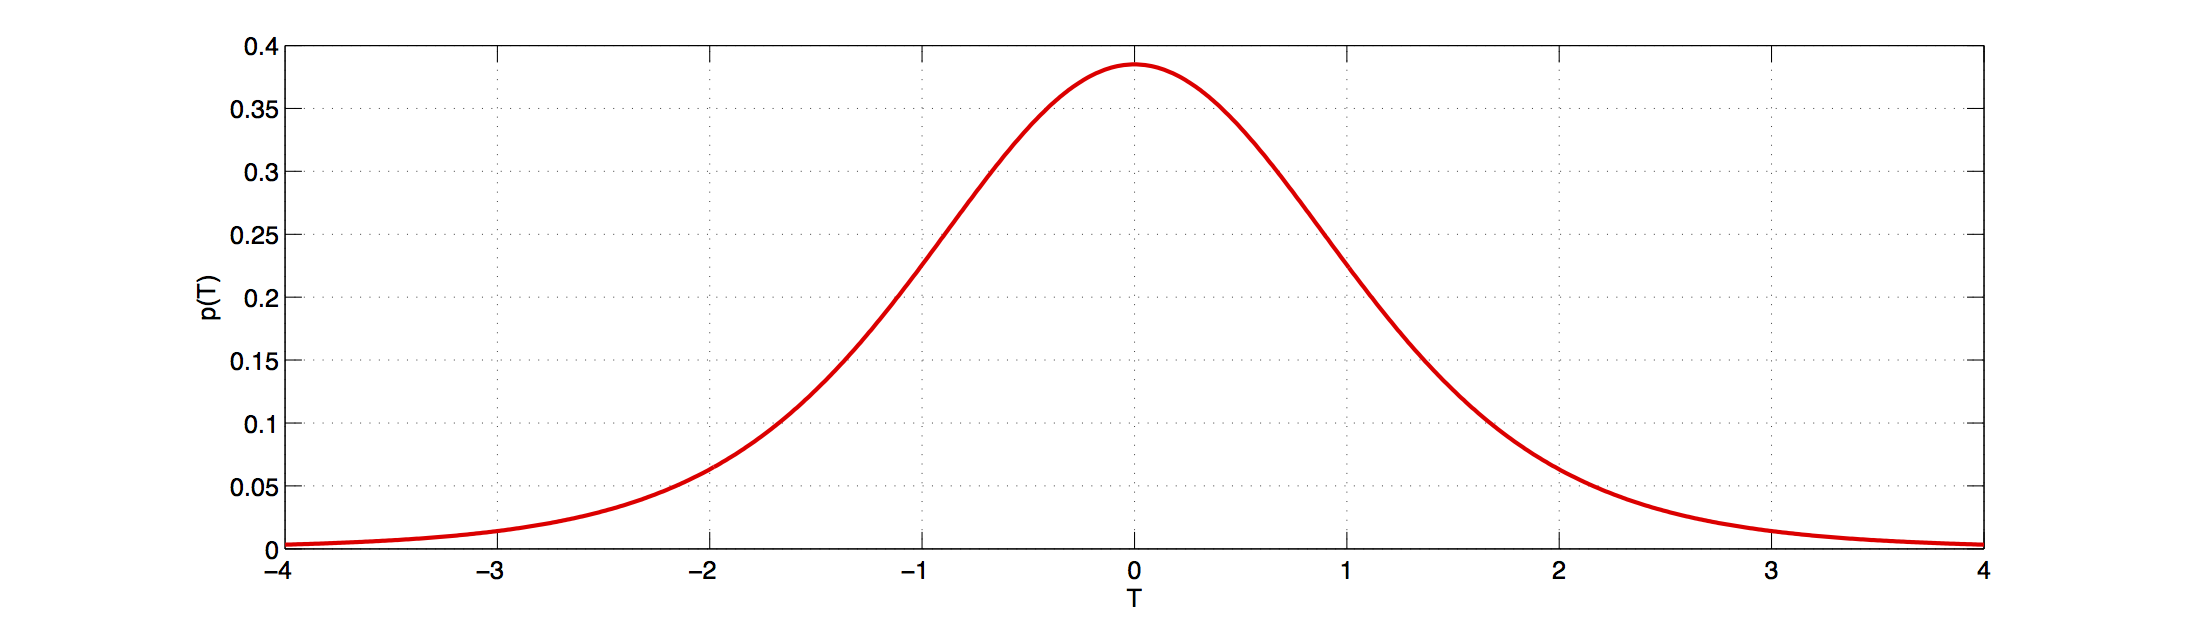
\includegraphics[width=0.8\textwidth]{stud.png}
		\end{center}
\end{frame}
\begin{frame}{Преобразование Фишера}
	\only<1>{
    \textbf{Стандартная ошибка:}
\[
    \text{SE} = \frac{\sigma}{\sqrt{n}},
\]    
для t-критерия:
\[
    \text{SE} = \frac{1-\hat{r}_{X_1X_2}^2}{\sqrt{n-2}}.
\]

Преобразование Фишера:
\[
    {z} = \text{arctanh}(\hat{r}_{X_1X_2}), \quad z \sim \mathcal{N}%(r_{X_1X_2}, \frac{n}{n-3}),
\]
\[
    \text{SE} = \frac{1}{\sqrt{n-3}}.
\]
}

	\only<2>{
		Доверительный интервал для коэффициента корреляции Пирсона:
		$$\left[  \hat{r}_{X_1X_2} + \frac{ t_{n-2, \alpha/2} \left(1-\hat{r}_{X_1X_2}^2\right)}{\sqrt{n}}, \hat{r}_{X_1X_2}- \frac{t_{n-2, \alpha/2} \left(1-\hat{r}_{X_1X_2}^2\right)}{\sqrt{n}} \right].$$
		
		\bigskip
		
		C использованием преобразования Фишера:
		$$\left[ \tanh\left(\arctanh \hat{r}_{X_1X_2} + \frac{z_{\alpha/2}}{\sqrt{n-3}}\right), \tanh \left( \arctanh \hat{r}_{X_1X_2} - \frac{z_{\alpha/2}}{\sqrt{n-3}} \right) \right].$$
		
	}
	
	\only<3>{
		\begin{block}{Пример, Kanji, критерий 12} Для двух марок зубной пасты, одна~из которых рекламируется по телевизору, а другая нет, участники опроса (30~человек) выставляют оценки в баллах от 1 до 20 в соответствии со~своими предпочтениями. Коэффициент корреляции Пирсона между оценками двух марок составляет 0.32, значимо ли эта величина отличается от нуля?
        \end{block}
		
		\bigskip
		
		$H_0\colon r_{X_1X_2}=0$
		
		$H_1\colon r_{X_1X_2}\neq 0$
		
		Критерий Стьюдента: $p = 0.0847.$
		
		\bigskip
		
		Доверительный интервал: $\left[-0.0157,0.6557\right].$
		
		C использованием преобразования Фишера: $\left[-0.0455,0.6100\right].$
	}
\end{frame}

\begin{frame}{Перестановочный критерий}
	\only<1>{
		\begin{center}
			\begin{tabular}{rl}
				выборки:                        & $X_1^n=\left(X_{11},\ldots,X_{1n}\right)$\\
				                                & $X_2^n=\left(X_{21},\ldots,X_{2n}\right)$\\
				                                & выборки связанные\\
				нулевая гипотеза:               & $H_0\colon r_{X_1X_2}=0$ \\
				альтернатива:                   & $H_1\colon r_{X_1X_2}<\neq>0$ \\
				статистика:                     & $T\left(X_1^n, X_2^n\right) = \hat{r}_{X_1X_2}$ \\
				нулевое распределение:          & порождается перебором $n!$ перестановок  \\
												& индексов одной из выборок
			\end{tabular}
		\end{center}		
 Достигаемый уровень значимости~--- доля перестановок, на которых получилось такое же или ещё более экстремальное значение статистики.
	}
	
	\only<2>{
%			Перестановочный $100(1-\alpha)$-\% доверительный интервал для коэффициента корреляции образован выборочными квантилями порядка $\alpha/2$ и $1-\alpha/2$ перестановочного распределения $T\left(X_1^n, gX_2^n\right).$
%			
%			\bigskip
%			
%			\bigskip
		
        \begin{block}{Пример, Kanji, критерий 12} Для двух марок зубной пасты, одна~из которых рекламируется по телевизору, а другая нет, участники опроса (30~человек) выставляют оценки в баллах от 1 до 20 в соответствии со~своими предпочтениями. Коэффициент корреляции Пирсона между оценками двух марок составляет 0.32, значимо ли эта величина отличается от нуля?
        \end{block}
		
        
		$ \hat{r}_{X_1X_2} =0.32 $
		
		$H_0\colon r_{X_1X_2}=0$
		
		$H_1\colon r_{X_1X_2}\neq 0$
		
		Критерий Стьюдента: $p = 0.0847.$		
				
		Перестановочный критерий: $p = 0.0564.$
	}
\end{frame}

\subsection{r Спирмена}
\begin{frame}{Корреляция Спирмена}
%%%%%%%%%%%%%%%%%%%%%%%%%%%%%%%%%%%%%%%%%%%%%%%%%%%%%%%%%%%%%%%%%%%%%%%
% Коэффициент корреляции Спирмена — это мера силы монотоннои? взаимосвязи между двумя случаи?ными величинами, он равен коэффициенту корреляции Пирсона между рангами наблюдении?. Для того, чтобы ее посчитать, нужно выборку пар (X1i , X2i ) , i = 1, . . . , n превратить наблюдение в каждои? из подвыборок в ранги rank (X1i ) , взять rank(X2i), и уже на этих рангах посчитать значение коэффициента корреляции Пирсона. Именно за счет рангового преобразования получается, что корреляция Спирмена чувствительна к любои? монотоннои? взаимосвязи между X1 и X2, поскольку ранговое преобразование превращает любую монотонную взаимосвязь в линеи?ную.
%%%%%%%%%%%%%%%%%%%%%%%%%%%%%%%%%%%%%%%%%%%%%%%%%%%%%%%%%%%%%%%%%%%%%%%
	\only<1>{
		\textbf{Коэффициент корреляции Спирмена} $\rho_{X_1X_2}$ случайных величин $X_1$ и~$X_2$~--- мера силы \textbf{монотонной} корреляции между ними; равен коэффициенту корреляции Пирсона между рангами наблюдений.
		
		\bigskip
		
		Выборочный коэффициент корреляции Спирмена:
		\begin{align*}
		\hat{\rho}_{X_1X_2} &= \frac{ \sum\limits_{i=1}^n \left(\rank\left(X_{1i}\right) - \frac{n+1}{2}\right)\left(\rank\left(X_{2i}\right) - \frac{n+1}{2}\right) }{\frac1{12}\left(n^3-n\right)} = \\
		&= 1-\frac{6}{n^3-n} \sum\limits_{i=1}^n \left(\rank\left(X_{1i}\right) - \rank\left(X_{2i}\right)\right)^2,
		\end{align*}
		$\rank\left(X_{1i}\right), \rank\left(X_{2i}\right)$ --- ранги $i$-х наблюдений в соответствующих выборках.
		
	}
	
	\only<2>{
%%%%%%%%%%%%%%%%%%%%%%%%%%%%%%%%%%%%%%%%%%%%%%%%%%%%%%%%%%%%%%%%%%%%%%%
%  Чтобы посмотреть, какие из свои?ств корреляции Спирмена отличаются от свои?ств корреляции Пирсона, можно воспроизвести эксперименты с облаками точек. Корреляция Спирмена примерно так же, как и корреляция Пирсона, реагирует на сжатие и размывание облака точек на диаграмме рассеяния). Видно, что краи?ние случаи идеальнои? линеи?нои? взаимосвязи соответствуют ?1 и 1, а в середине получаются значения коэффициента корреляции, близкие к 0.
% Более интересные результаты получаются в эксперименте с загибанием облака точек. Видно, что пока зависимость между X1 и X2 остается монотоннои? (рисунки 8.6a, 8.6b), значение коэффициента корреляции Спирмена почти не убывает 1. Однако потом, когда облако точек начинает превращаться в параболу, значение выборочного коэффициента корреляции Спирмена постепенно превращается в 0. Корреляция Спирмена не обнаруживает взаимосвязи между X1 и X2, отличные от монотонных. Это можно заметить и на следующих примерах. Когда между X1 и X2 есть какие-то сложные функциональные взаимосвязи, корреляция Спирмена все равно остается близкои? к 0, поскольку они далеки от монотонных.
% Гораздо более интересные результаты получаются в эксперименте с выбросами. Когда из облака точек с сильнои? отрицательнои? корреляциеи? пять точек начинают выдвигаться в правыи? верхнии? угол диаграммы рассеяния, значение коэффициента корреляции Спирмена сначала немного уменьшается. Однако как только эти пять точек оказываются за пределами диапазона изменении? случаи?ных величин в основном облаке, значение коэффициента корреляции Спирмена меняться перестает. Как бы далеко они ни отодвигались, не удае?тся получить большую положительную корреляцию, как в случае с корреляциеи? Пирсона. Это говорит о том, что коэффициент корреляции Спирмена гораздо более устои?чив к выбросам, то есть, небольшое количество точек с нетипичными значениями признаков очень слабо влияют на выборочное значение коэффициента корреляции.
%%%%%%%%%%%%%%%%%%%%%%%%%%%%%%%%%%%%%%%%%%%%%%%%%%%%%%%%%%%%%%%%%%%%%%%
		\begin{center}
			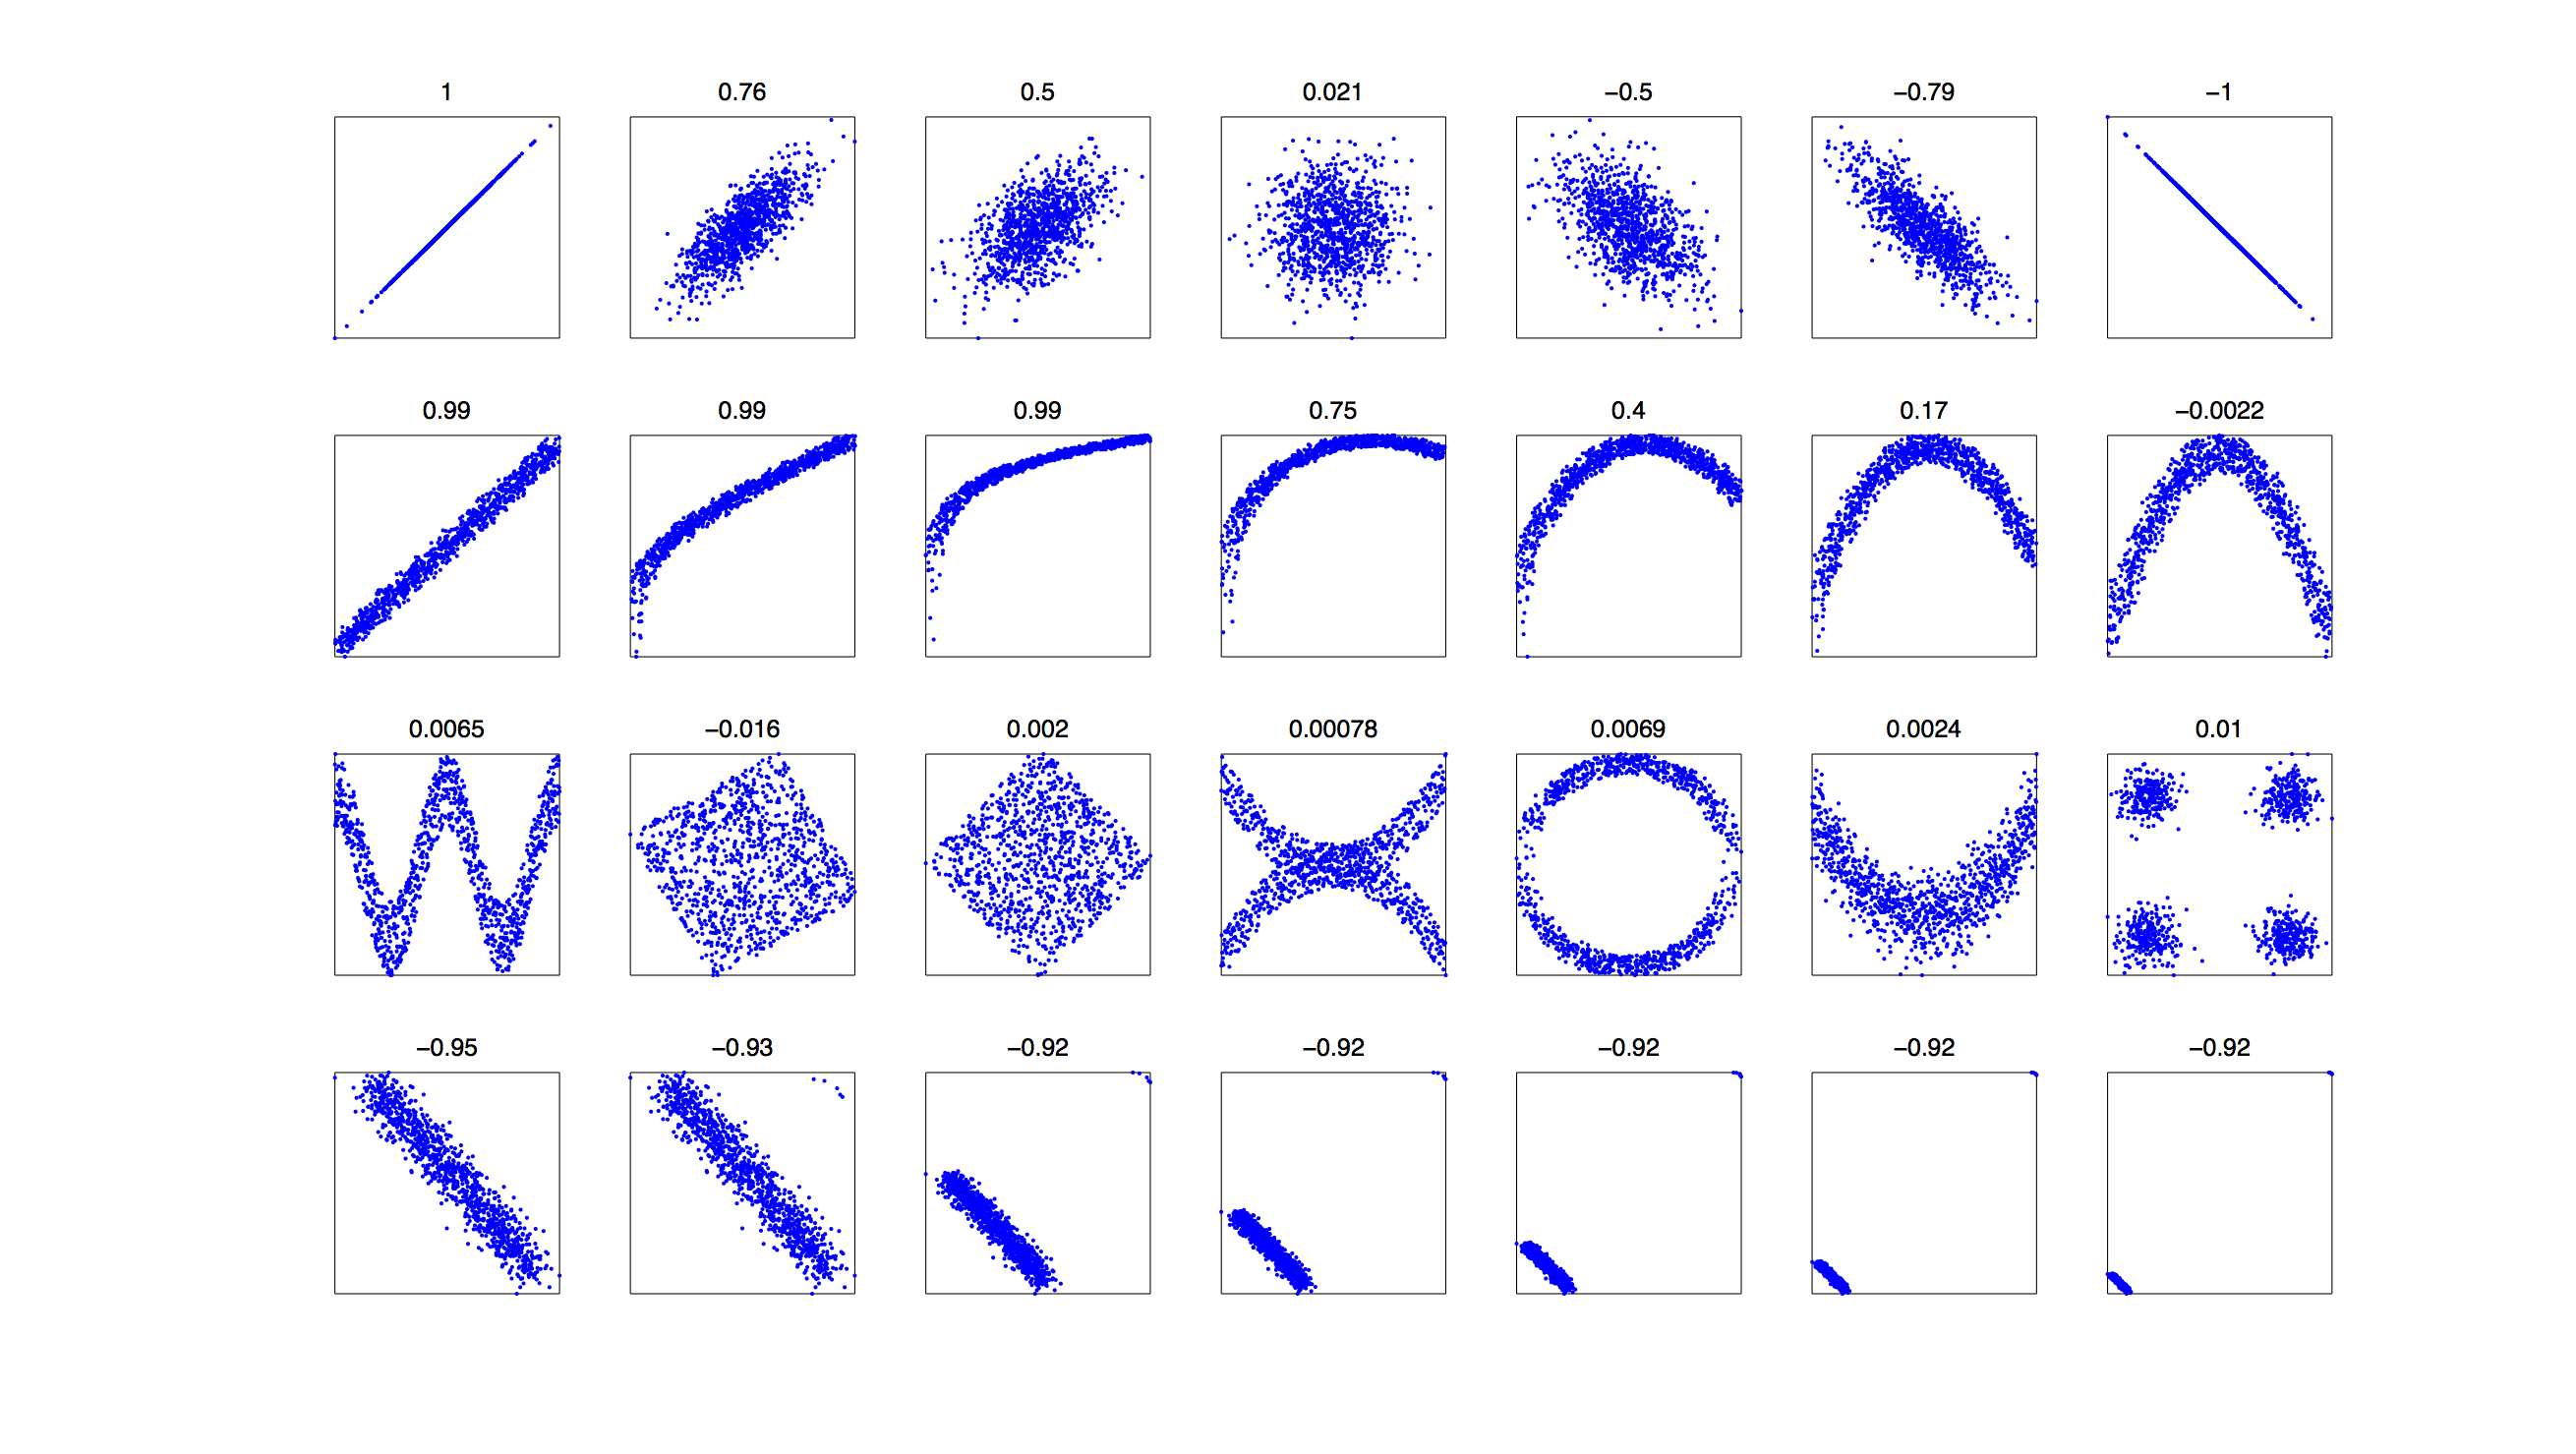
\includegraphics[width=0.8\textwidth]{corr_spearman.png}
		\end{center}
	}
\end{frame}

\begin{frame}{Критерий Стьюдента}
	\only<1>{
		\begin{center}
			\begin{tabular}{rl}
				выборки:                        & $X_1^n=\left(X_{11},\ldots,X_{1n}\right)$\\
				                                & $X_2^n=\left(X_{21},\ldots,X_{2n}\right)$\\
				                                & выборки связанные\\
				нулевая гипотеза:               & $H_0\colon \rho_{X_1X_2}=0$ \\
				альтернатива:                   & $H_1\colon \rho_{X_1X_2}<\neq>0$ \\
				статистика:                     & $T\left(X_1^n, X_2^n\right) = \frac{\hat{\rho}_{X_1X_2} \sqrt{n-2}}{\sqrt{1-\rho^2_{X_1X_2}}}$ \\
				нулевое распределение:          & $St(n-2)$\\
			\end{tabular}
			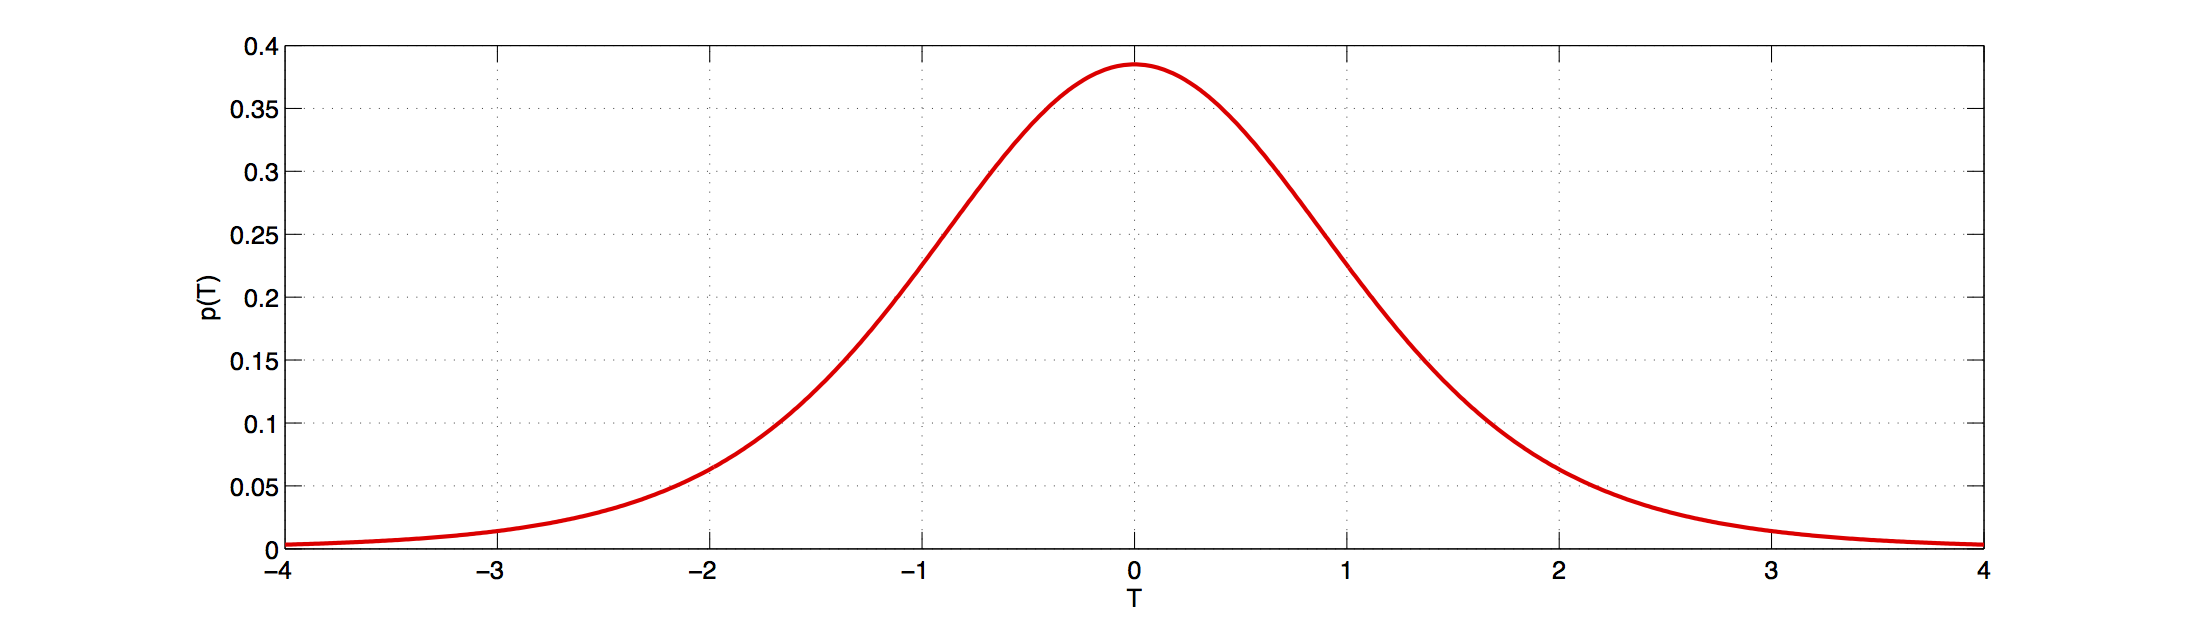
\includegraphics[width=0.8\textwidth]{stud.png}
		\end{center}
	}
	
	\only<2>{
		\begin{block}{Пример,Kanji, критерий 58}Выборка из 11 потребителей вегетариантских сосисок оценивает качество двух брендов. Если целевая аудитория двух брендов совпадает, то их рекламу можно давать совместно. Корреляция Спирмена оценок потребителей равна $-0.854$
		\end{block}
		\bigskip
		
		$H_0\colon \rho_{X_1X_2}=0$
		
		$H_1\colon \rho_{X_1X_2}\neq 0$
		
		Критерий Стьюдента: $p = 0.0024.$
	}
\end{frame}

\subsection{t Кендалла}
\begin{frame}{Корреляция Кендалла}
	\only<1>{
		\textbf{Коэффициент корреляции Кендалла} $\tau_{X_1X_2}$ случайных величин $X_1$ и~$X_2$~--- мера их взаимной неупорядоченности; также оценивает силу \textbf{монотонной} корреляции между величинами. 
		
		\bigskip
		
		Выборочный коэффициент корреляции Кендалла:
		
		
		$$\hat{\tau}_{X_1X_2} = 1 - \frac{4}{n\left(n-1\right)} \sum_{i=1}^{n-1} \sum_{j=1}^n \left[\left[X_{1i}<X_{1j}\right]\neq\left[X_{2i}<X_{2j}\right]\right] = \frac{C-D}{C+D},$$
		где $C$ --- число согласованных пар, $D$ --- число несогласованных пар.
	}
	
	\only<2>{
		\begin{center}
			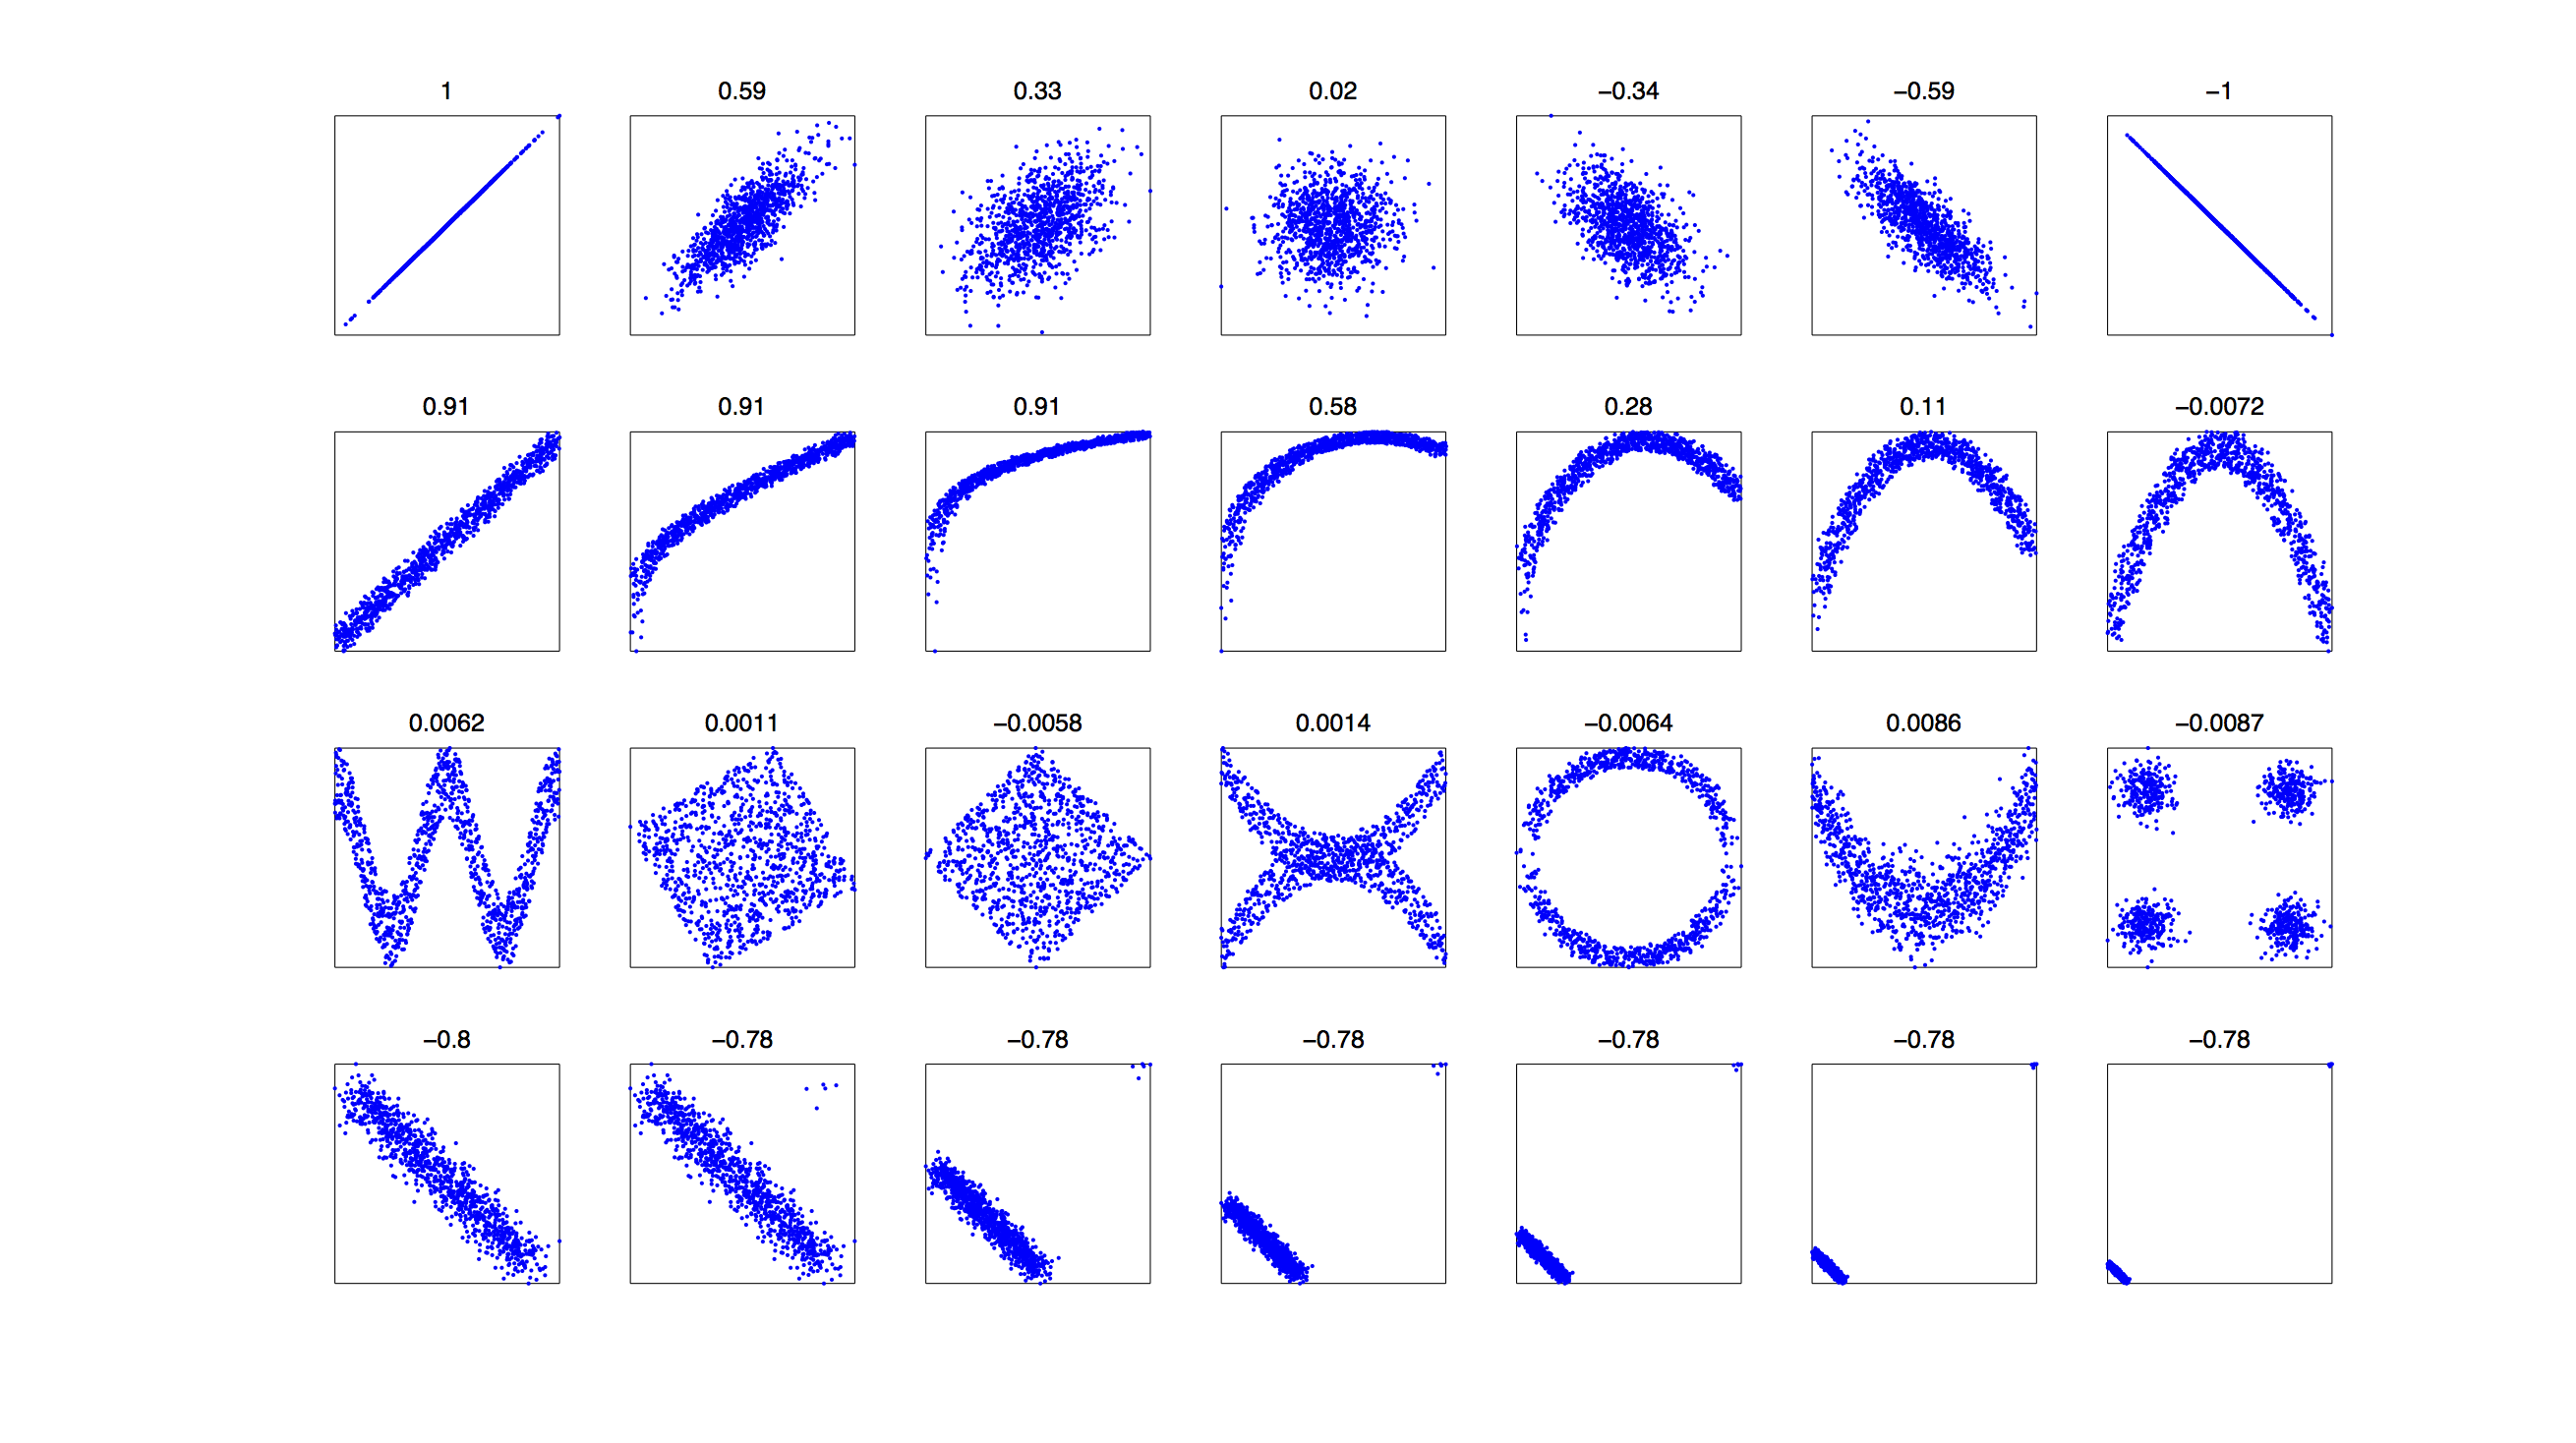
\includegraphics[width=0.8\textwidth]{corr_kendall.png}
		\end{center}
	}
\end{frame}

\begin{frame}{Критерий без названия}
	\only<1>{
		\begin{center}
			\begin{tabular}{rl}
				выборки:                        & $X_1^n=\left(X_{11},\ldots,X_{1n}\right)$\\
				                                & $X_2^n=\left(X_{21},\ldots,X_{2n}\right)$\\
				                                & выборки связанные\\
				нулевая гипотеза:               & $H_0\colon \tau_{X_1X_2}=0$ \\
				альтернатива:                   & $H_1\colon \tau_{X_1X_2}<\neq>0$ \\
				статистика:                     & $\hat{\tau}_{X_1X_2}$ \\
				нулевое распределение:          & табличное\\
			\end{tabular}
		\end{center}
		
		\bigskip
		
		При справедливости $H_0$
		$$\mathbb{E}\hat{\tau}_{X_1X_2} = 0, \;\; \mathbb{D}\hat{\tau}_{X_1X_2} = \frac{2\left(2n+5\right)}{9n\left(n-1\right)}.$$
		
		\bigskip
		
		Для $n>10$ справедлива аппроксимация нормальным распределением.
	}
	
	\only<2>{
		\begin{block}{Пример,Kanji, критерий 59} Налоговый инспектор хочет проверить наличие взаимосвязи между величинами общего дохода от инвестиций и~общего объёма дополнительных доходов. На выборке из 10 налоговых деклараций он получил $D=5, \; C=38, \; \hat{\tau}_{X_1X_2}=0.7821.$
		\end{block}
		\bigskip
		
		$H_0\colon \tau_{X_1X_2}=0.$
		
		$H_1\colon \tau_{X_1X_2}\neq 0 \Rightarrow p = 0.0027.$
	}
\end{frame}

\begin{frame}{Связь между коэффициентами корреляции}
	При справедливости $H_0$ (отсутствии монотонной зависимости):
	
	\begin{minipage}{0.39\textwidth}
		$r_{\rho_{X_1X_2}\tau_{X_1X_2}} = \frac{2n+2}{\sqrt{4n^2+10n}}$
	\end{minipage}%
	\begin{minipage}{0.6\textwidth}
		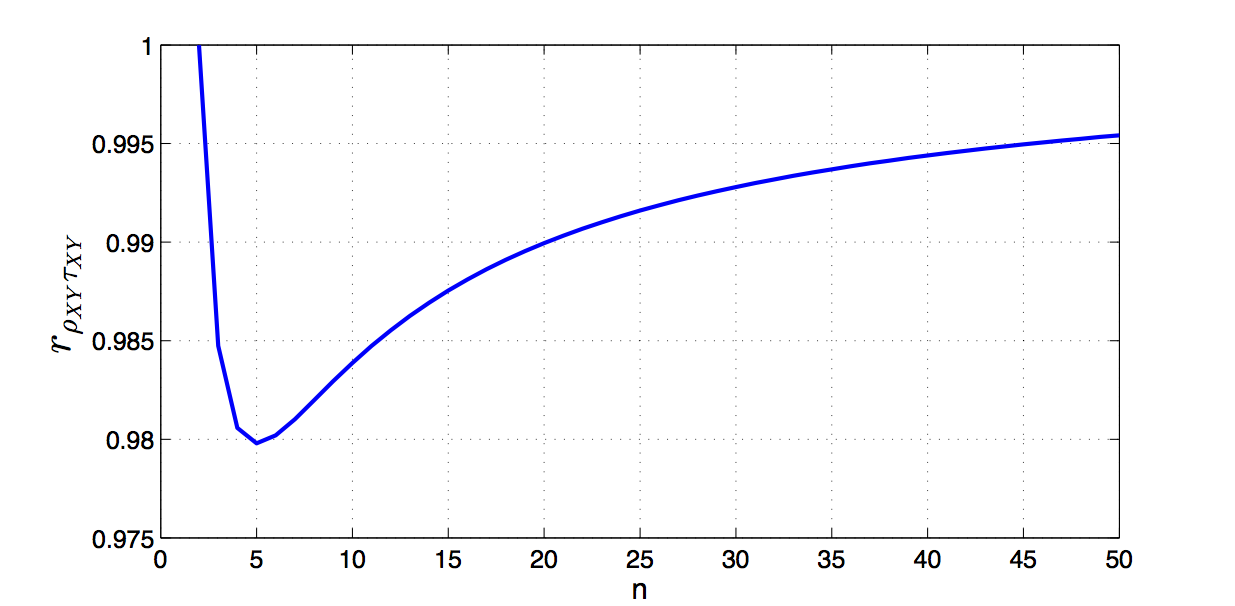
\includegraphics[width=0.8\textwidth]{corrcorr.png}
	\end{minipage}
	
	\vspace{5pt}
	
	\url{http://youtu.be/D56dvoVrBBE}: по сравнению с корреляцией Спирмена, корреляция Кендалла
	\begin{itemize}
		\item менее чувствительна к большим различиям между рангами наблюдений;
		\item точнее оценивается по выборке небольших объёмов;
		\item обычно меньше по модулю.
	\end{itemize}
	
	$$\left(X_{1},X_{2}\right)\sim N\left(\mu,\Sigma\right) \;\; \Rightarrow\;\;\lim_{n\rightarrow\infty} \mathbb{E} \tau_{X_1X_2} = \lim_{n\rightarrow\infty} \mathbb{E} \rho_{X_1X_2} = \frac{2}{\pi} \arcsin r_{X_1X_2}.$$
\end{frame}

\subsection{Частная корреляция}
\begin{frame}{Частная корреляция}
	Если мы подозреваем, что наблюдаемая линейная взаимосвязь между признаками $X_1$ и $X_2$ вызвана влиянием третьего признака $X_3$, можно попытаться его снять.
	
	Частная корреляция:
	$$r_{X_1X_2|X_3} = \frac{r_{X_1X_2} - r_{X_1X_3} r_{X_2X_3}}{\sqrt{\left(1-r_{X_1X_3}^2\right)\left(1-r_{X_2X_3}^2\right)}}.$$
	
	Если нужно снять влияние нескольких признаков, можно пользоваться рекуррентной формулой:
	$$r_{X_1X_2|X_3X_4} = \frac{r_{X_1X_2|X_4} - r_{X_1X_3|X_4} r_{X_2X_3|X_4}}{\sqrt{\left(1-r_{X_1X_3|X_4}^2\right)\left(1-r_{X_2X_3|X_4}^2\right)}}.$$
	Другой вариант: если $M$ --- множество признаков, $\Omega$ --- обратимая матрица их выборочных корреляций, $R=\Omega^{-1},$ то
	$$r_{X_iX_j|M \setminus \{X_i,X_j\}} = - \frac{r_{ij}}{\sqrt{r_{ii}r_{jj}}}.$$
\end{frame}

\begin{frame}{Критерий Стьюдента}
	%\vspace{-10pt}
	\begin{center}
		\begin{tabular}{rl}
			выборки:                        & $X_1^n=\left(X_{11},\ldots,X_{1n}\right)$ \\
			                                & $X_2^n=\left(X_{21},\ldots,X_{2n}\right)$\\
			                                & $X_3^n=\left(X_{31},\ldots,X_{3n}\right), X_{3} \in \mathbb{R}^M$\\
		  	                                & $\left(X_{1},X_{2},X_{3}\right)\sim N\left(\mu,\Sigma\right)$ \\
			нулевая гипотеза:               & $H_0\colon r_{X_1X_2|X_3}=0$ \\
			альтернатива:                   & $H_1\colon r_{X_1X_2|X_3}<\neq>0$ \\
			статистика:                     & $T\left(X_1^n, X_2^n, X_3^n\right) = \frac{\hat{r}_{X_1X_2|X_3} \sqrt{n-M-2}}{\sqrt{1-\hat{r}_{X_1X_2|X_3}^2}}$ \\
			нулевое распределение:          & $St(n-M-2)$\\
		\end{tabular}
		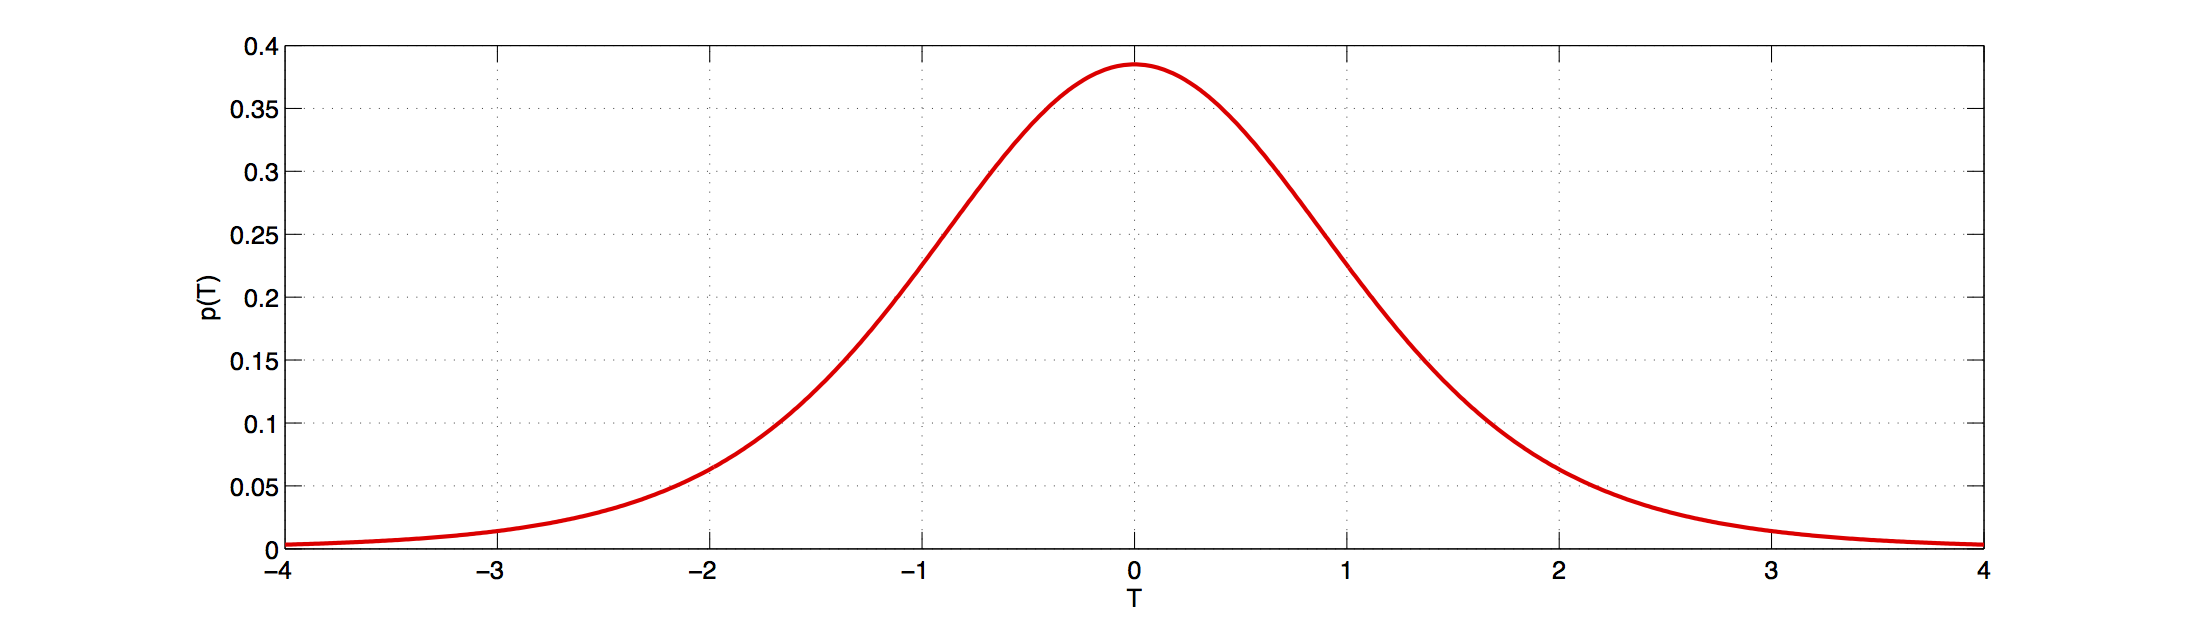
\includegraphics[width=\textwidth]{stud.png}
	\end{center}
\end{frame}

\subsection{Множественная корреляция}
\begin{frame}{Множественная корреляция}
	Для того, чтобы оценить силу линейной взаимосвязи одной переменной ($X_1$) с несколькими другими ($X_2,X_3$), используется множественная корреляция:
	$$r_{X_1,X_2,X_3} = \frac{r_{X_1X_2}^2 + r_{X_1X_3}^2 - 2r_{X_1X_2}r_{X_1X_3}r_{X_2X_3}}{1-r_{X_2X_3}^2}.$$
	
	Для большего числа признаков: пусть $M$ --- множество дополнительных признаков, $\Omega$ --- обратимая матрица их выборочных корреляций, $R=\Omega^{-1},$ $c$~--- вектор корреляций основного признака $X$ с дополнительными; тогда
	$$r_{X,M}^2 = c^T Rc.$$
	
	\bigskip
	
	
	\bigskip
	
	$r_{X,M}\in[0,1].$
\end{frame}

\begin{frame}{Критерий Фишера}
	\begin{center}
		\begin{tabular}{rl}
			выборки:                        & $X_1^n=\left(X_{11},\ldots,X_{1n}\right)$\\
		  	                                & $X_2^n=\left(X_{21},\ldots,X_{2n}\right), X_{2} \in \mathbb{R}^M$\\
			                                & $\left(X_{1},X_{2}\right)\sim N\left(\mu,\Sigma\right)$ \\
			нулевая гипотеза:               & $H_0\colon r_{X_1,X_2}=0$ \\
			альтернатива:                   & $H_1\colon r_{X_1,X_2}>0$ \\
			статистика:                     & $F\left(X_1^n, X_2^n\right) = \frac{\hat{r}_{X_1,X_2}^2}{1-\hat{r}_{X_1,X_2}^2}\frac{n-M-1}{M-2}$ \\
			нулевое распределение:          & $F(M-2, n-M-1)$\\
		\end{tabular}
		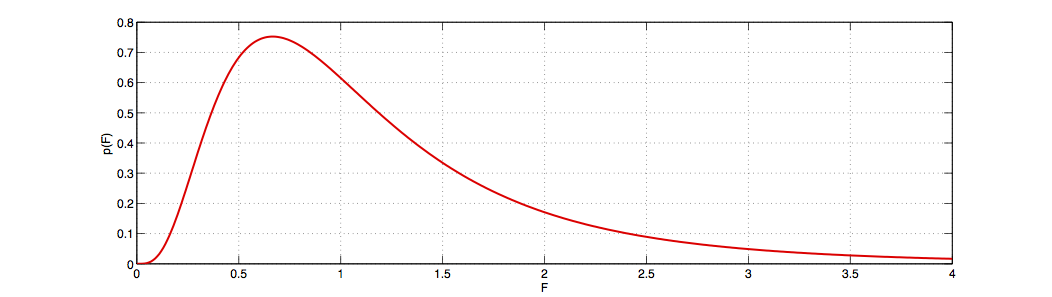
\includegraphics[width=0.8\textwidth]{fish.png}
	\end{center}
\end{frame}

\begin{frame}{Температура воздуха и географическое положение}
	\only<1>{
		По 56 городам США известны средняя минимальная температура января и географические координаты (широта, долгота). Требуется исследовать характер зависимости между переменными.
		
		\begin{center}
			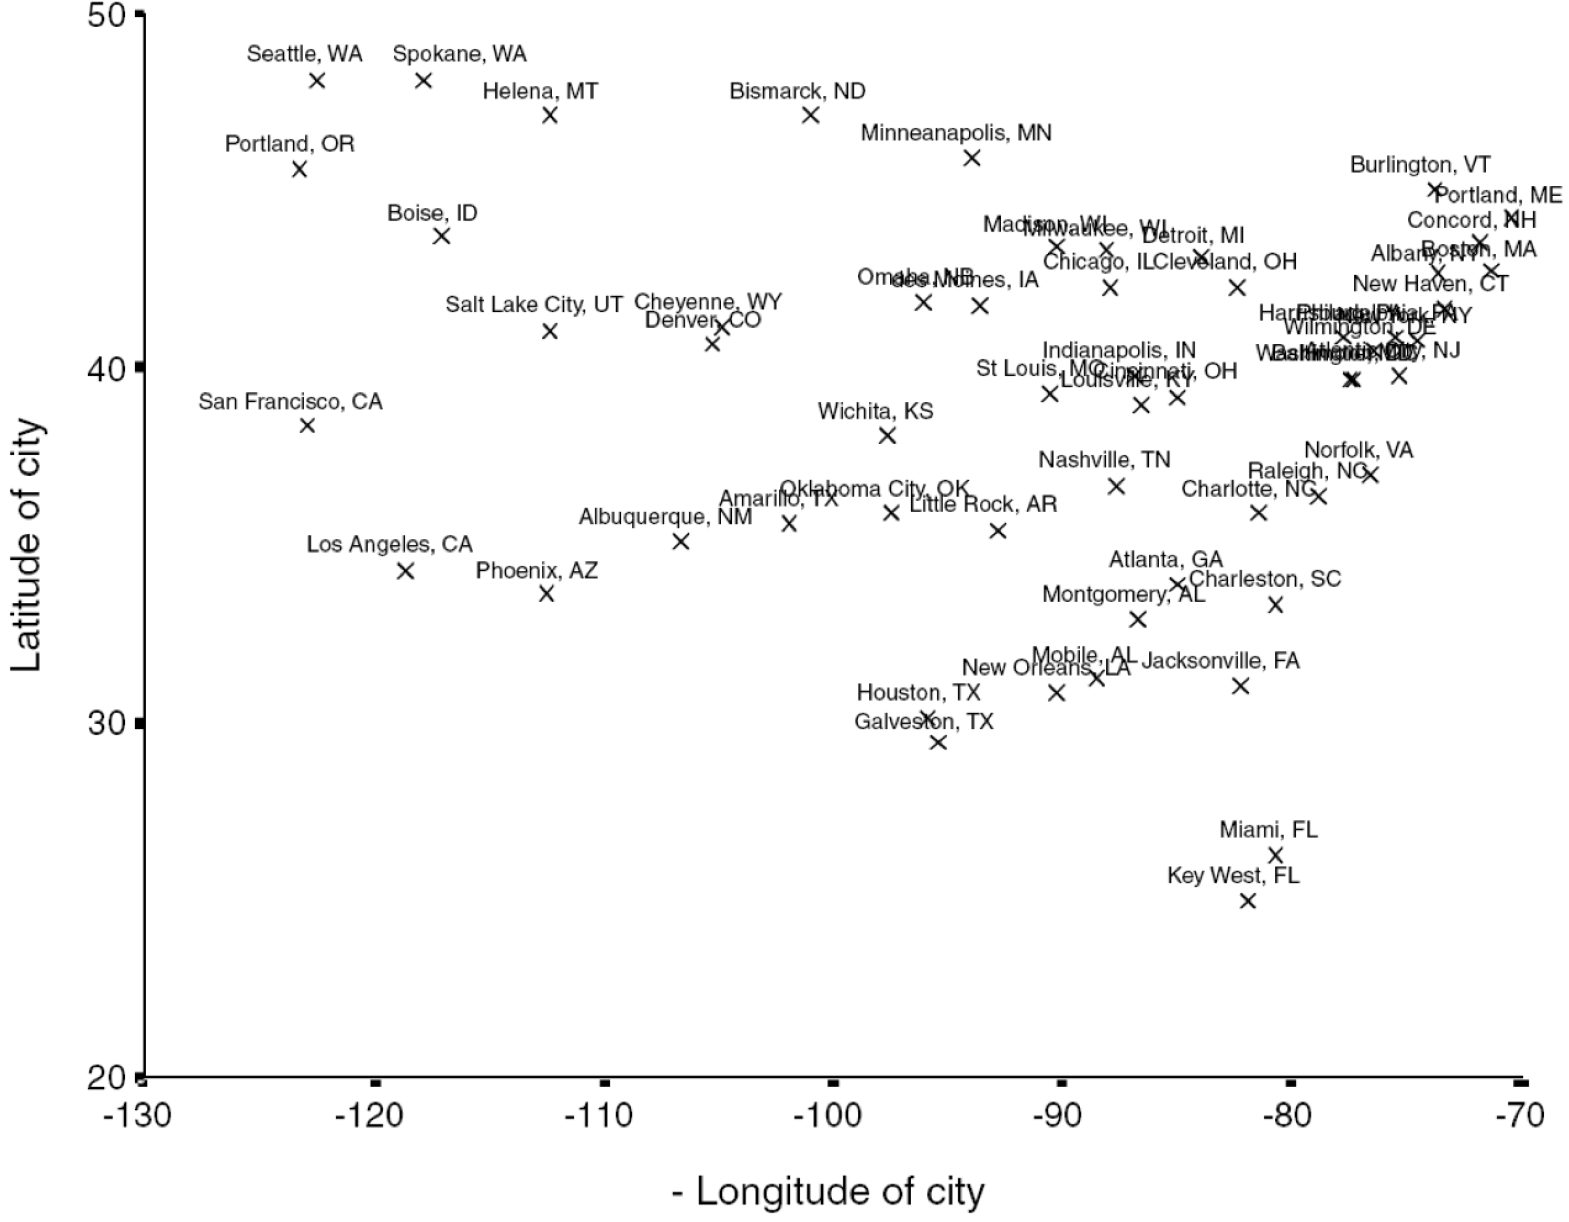
\includegraphics[height=0.7\textheight]{mapped.png}
		\end{center}
	}
	
	\only<2>{
		\begin{center}
			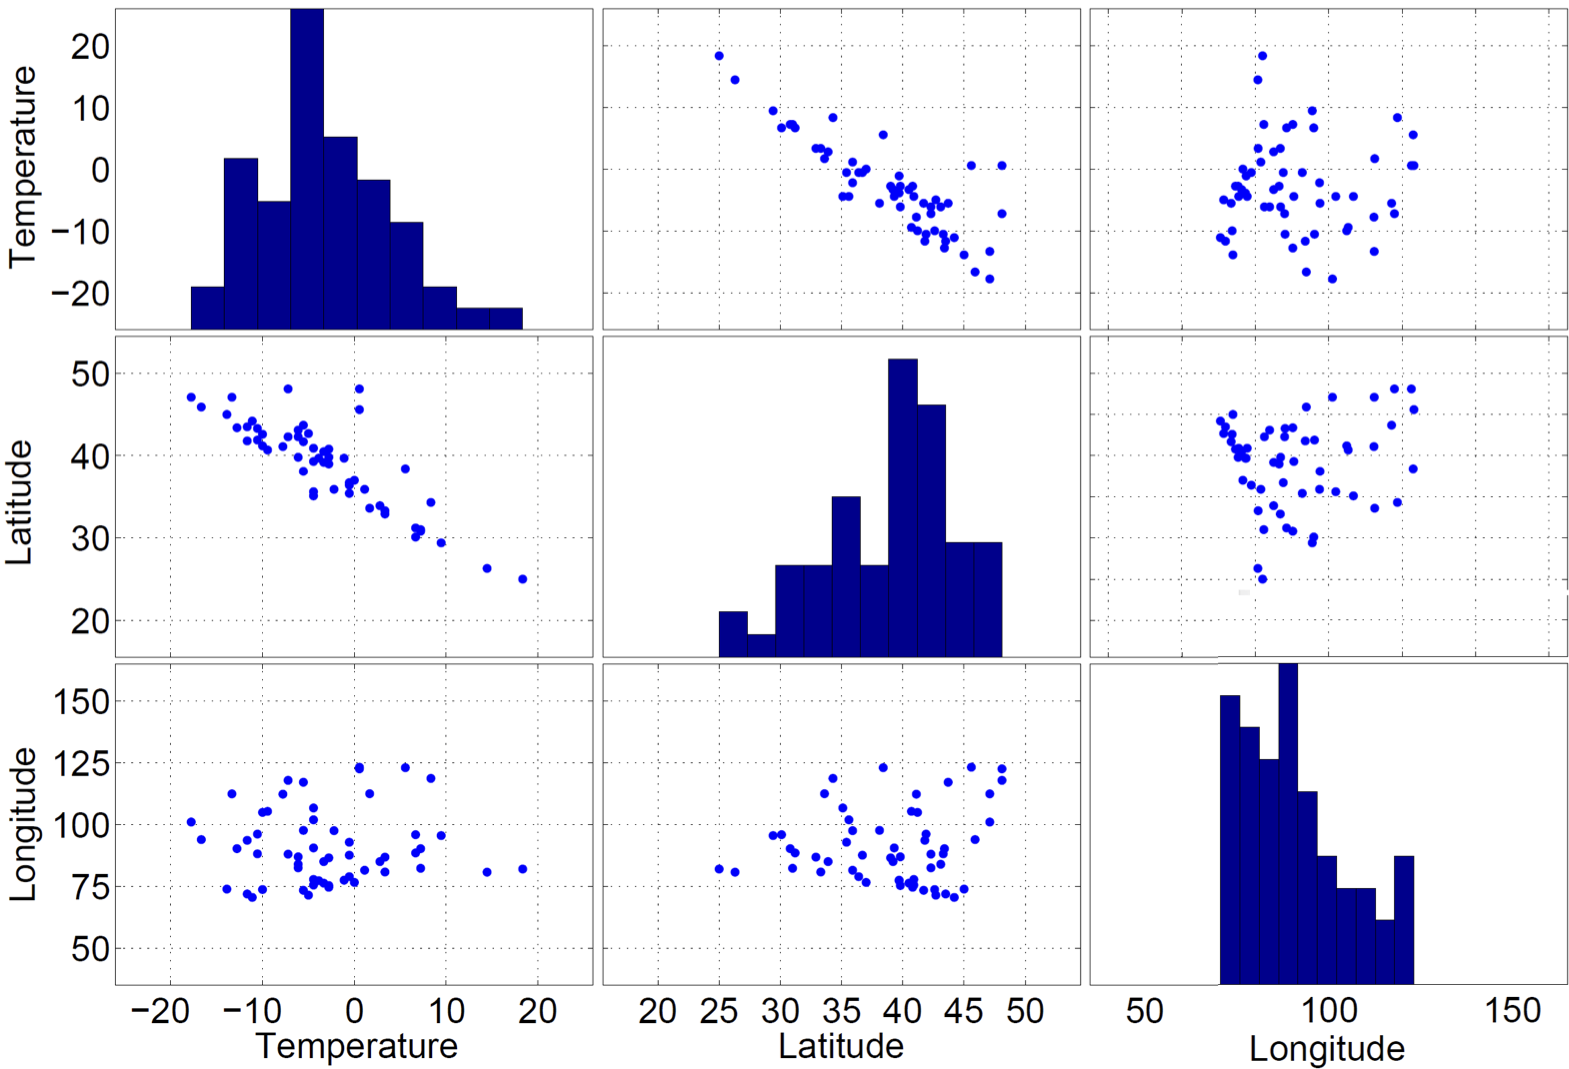
\includegraphics[width=0.7\textwidth]{temperature.png}
		\end{center}
	}
	
	\only<3>{
		$T$~--- температура, $\lambda$~--- долгота, $\phi$~--- широта;
		
		$r$~--- корреляция Пирсона, $\rho$~--- Спирмена, $\tau$~--- Кендалла.
		
		\bigskip
		
		Коэффициенты корреляции:
		\begin{center}\scriptsize
			\setlength{\tabcolsep}{2pt}
			\begin{tabular}{|>{$}r<{$}|>{$}r<{$} >{$}r<{$} >{$}r<{$}|} \hline
				r       &T                   &\phi                &\lambda \\ \hline
				T       &-                   &\boldsymbol{-0.848} &0.024   \\
				\phi    &\boldsymbol{-0.848} &-                   &0.145   \\
				\lambda &0.024               &0.145               &-       \\\hline
			\end{tabular}
			\quad
			\begin{tabular}{|>{$}r<{$}|>{$}r<{$} >{$}r<{$} >{$}r<{$}|} \hline
				\tau    &T                   &\phi                & \lambda \\ \hline
				T       &-                   &\boldsymbol{-0.683} & 0.030      \\
				\phi    &\boldsymbol{-0.683} &-                   & -0.011     \\
				\lambda &0.030               &-0.011              & -    \\\hline
			\end{tabular}
			\quad
			\begin{tabular}{|>{$}r<{$}|>{$}r<{$} >{$}r<{$} >{$}r<{$}|} \hline
				\rho    & T                   & \phi                & \lambda \\ \hline
				T       & -                   & \boldsymbol{-0.815} & 0.030    \\
				\phi    & \boldsymbol{-0.815} & -                   & 0.023    \\
				\lambda & 0.030               & 0.023               & -        \\ \hline
			\end{tabular}
		\end{center}
		
		\bigskip
		
		Достигаемые уровни значимости:
		\begin{center}\scriptsize
			\setlength{\tabcolsep}{2pt}
			\begin{tabular}{|>{$}r<{$}|>{$}r<{$} >{$}r<{$} >{$}r<{$}|} \hline
				r       &T                   &\phi                &\lambda \\ \hline
				T       & -                  & \boldsymbol{0.000} & 0.861    \\
				\phi    & \boldsymbol{0.000} & -                  & 0.287 \\
				\lambda & 0.861              & 0.287              & - \\\hline
			\end{tabular}
			\quad
			\begin{tabular}{|>{$}r<{$}|>{$}r<{$} >{$}r<{$} >{$}r<{$}|} \hline
				\tau    &T                   &\phi                &\lambda \\ \hline
				T       & -                  & \boldsymbol{0.000} & 0.756\\
				\phi    & \boldsymbol{0.000} & -                  & 0.910 \\
				\lambda & 0.756              & 0.910              & -   \\\hline
			\end{tabular}
			\quad
			\begin{tabular}{|>{$}r<{$}|>{$}r<{$} >{$}r<{$} >{$}r<{$}|} \hline
				\rho    &T                   &\phi                &\lambda \\ \hline
				T       & -                  & \boldsymbol{0.000} & 0.829    \\
				\phi    & \boldsymbol{0.000} & -                  & 0.865    \\
				\lambda & 0.829              & 0.865              &  -       \\     \hline
			\end{tabular}
		\end{center}
	}
	
	\only<4>{
		$T$~--- температура, $\lambda$~--- долгота, $\phi$~--- широта;
		
		$r$~--- частная корреляция Пирсона, $\rho$~--- Спирмена.
		
		\bigskip
		
		Коэффициенты частной корреляции:
		\begin{center}\setlength{\tabcolsep}{2pt}
			\begin{tabular}{|>{$}r<{$}|>{$}r<{$} >{$}r<{$} >{$}r<{$}|} \hline
				r       &T                    &\phi                 &\lambda \\ \hline
				T       & -                   & \boldsymbol{-0.861} & \boldsymbol{0.280}    \\
				\phi    & \boldsymbol{-0.861} & -                   & \boldsymbol{0.312} \\
				\lambda & \boldsymbol{0.280}  & \boldsymbol{0.312}  & - \\\hline
			\end{tabular}
			\quad
			\begin{tabular}{|>{$}r<{$}|>{$}r<{$} >{$}r<{$} >{$}r<{$}|} \hline
				\rho    &T                    &\phi                 &\lambda \\ \hline
				T       & -                   & \boldsymbol{-0.817} & 0.084\\
				\phi    & \boldsymbol{-0.817} & -                   & 0.082 \\
				\lambda & 0.084               & 0.082               & -   \\\hline
			\end{tabular}
		\end{center}
		
		\bigskip
		
		Достигаемые уровни значимости:
		\begin{center}\setlength{\tabcolsep}{2pt}
			\begin{tabular}{|>{$}r<{$}|>{$}r<{$} >{$}r<{$} >{$}r<{$}|} \hline
				r       &T                   &\phi                &\lambda \\ \hline
				T       & -                  & \boldsymbol{0.000} & \boldsymbol{0.039}    \\
				\phi    & \boldsymbol{0.000} & -                  & \boldsymbol{0.021} \\
				\lambda & \boldsymbol{0.039} & \boldsymbol{0.021} & - \\\hline
			\end{tabular}
			\quad
			\begin{tabular}{|>{$}r<{$}|>{$}r<{$} >{$}r<{$} >{$}r<{$}|} \hline
				\rho    &T                   &\phi                &\lambda \\ \hline
				T       & -                  & \boldsymbol{0.000} & 0.543\\
				\phi    & \boldsymbol{0.000} & -                  & 0.552 \\
				\lambda & 0.543              & 0.552              & -   \\\hline
			\end{tabular}
		\end{center}
	}
	
	\only<5>{
		$T$~--- температура, $\lambda$~--- долгота, $\phi$~--- широта;
		
		$R$~--- множественная корреляция.
		
		\bigskip
		
		Коэффициенты множественной корреляции:
		\begin{center}
			\begin{tabular}{|r|ccc|}
				\hline
				& $T$                                & $\phi$                            & $\lambda$ \\ \hline
				$R$  & $0.659$                            & $0.667$                           & $0.312$     \\
				$p$  & $6.0347\times10^{-8}$              & $3.6481\times10^{-8}$             & $0.0216$    \\
				with & $0.235\cdot\lambda-0.638\cdot\phi$ & $ 0.397\cdot\lambda-0.678\cdot T$ & $1.542\cdot T+2.450\cdot \phi$  \\
				\hline
			\end{tabular}
		\end{center}
		
		\bigskip
		
		\begin{center}
			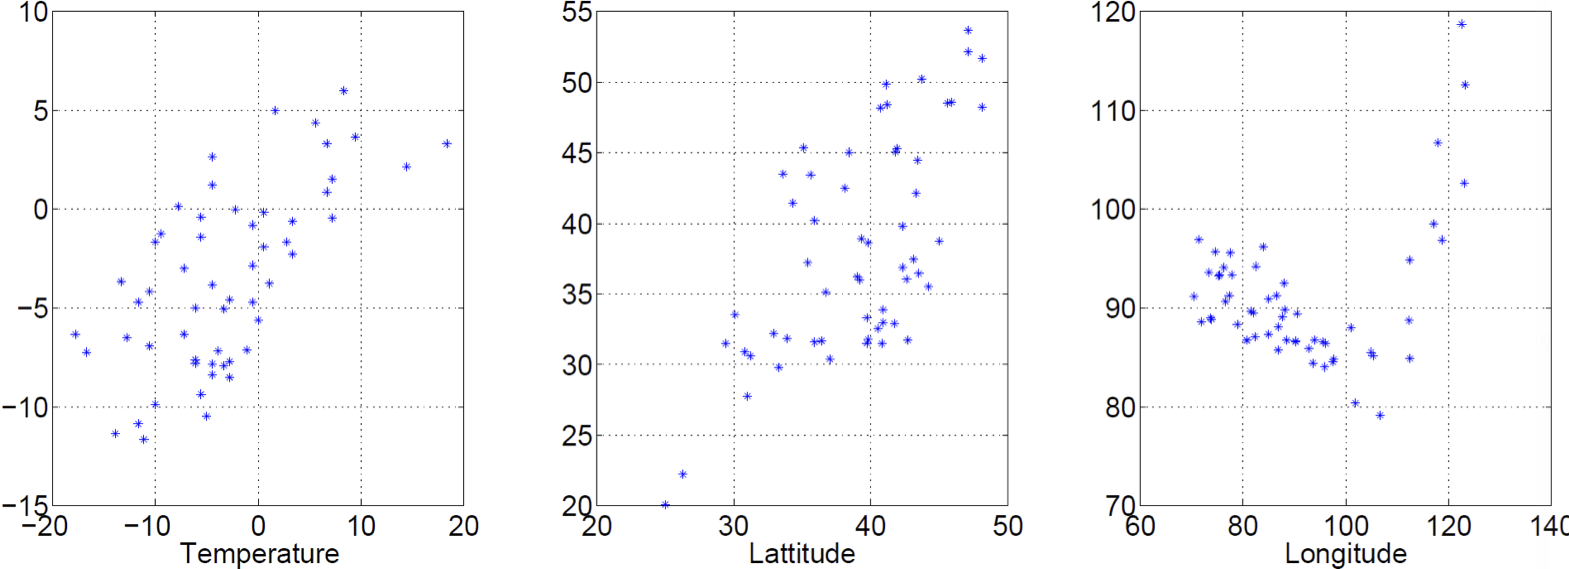
\includegraphics[width=0.8\textwidth]{multiple.png}
		\end{center}
	}
\end{frame}		

\section{Категориальные признаки}
\subsection{Таблицы сопряжённости}
\begin{frame}{Таблица сопряжённости $K_1 \times K_2$}
	Имеются связанные выборки $X_1^n = \left(X_{11},\ldots,X_{1n}\right)$ и $X_2^n = \left(X_{21},\ldots,X_{2n}\right)$, $X_{1} \in \left\{1,\dots,K_1\right\}$, $X_{2} \in \left\{1,\dots,K_2\right\}.$
	
	\bigskip
	
	Таблица сопряжённости:
	
	\begin{center}
		\begin{tabular}{|c|c|c|c|c|c|c|}
			\hline
			\diagbox{$X_1$}{$X_2$} & $1$ & $\ldots$ & $j$             & $\ldots$ & $K_2$ & $\sum$\\ \hline
			$1$                         &     &          &                 &          &       &   \\ \hline
			$\vdots$                    &     &          &                 &          &       &\\ \hline
			$i$                         &     &          & $n_{ij}$        &          &       &$n_{i+}$\\ \hline
			$\vdots$                    &     &          &                 &          &       &\\ \hline
			$K_1$                       &     &          &                 &          &       &\\ \hline
			$\sum$                      &     &          & $n_{+j}$        &          &       & $n$ \\ \hline
		\end{tabular}
	\end{center}
\end{frame}

\begin{frame}{Два случайных признака}
	Пусть $\pi_{ij}$~--- вероятность реализации пары $\left(X_{1},X_{2}\right)$ в ячейке $\left(i,j\right).$
	
	$\left\{\pi_{ij}\right\}$~--- совместное распределение $\left(X_{1},X_{2}\right);$
	
	$\left\{\pi_{i+}\right\}, \left\{\pi_{+j}\right\}$~--- маргинальные распределения:
    $$
    \left\{\pi_{i+}\right\} = \sum_{j=1}^{K_2}\pi_{ij},  
    $$
    $$
    \left\{\pi_{+j}\right\} = \sum_{i=1}^{K_1}\pi_{ij}.
    $$
	
	\bigskip
	
	$X_1$ и $X_2$ независимы, если
	$$\pi_{ij} = \pi_{i+}\pi_{+j} \;\; \forall i=1,\dots,K_1, j=1,\dots,K_2.$$
\end{frame}

\begin{frame}{Один случайный признак}
	Пусть $X_{1}$~--- не случайная величина, а фиксированный признак.
	Тогда $\left\{\pi_{ij}\right\}$ не имеет смысла, вместо него рассматриваются $\left\{\pi_{1|i},\dots,\pi_{K_1|i}\right\}$~--- условные распределения $X_2$ при $X_1=i.$
	
	\bigskip
	
	$X_1$ и $X_2$ независимы, если
	$$\pi_{j|1} = \dots = \pi_{j|K_1} \;\; \forall j=1,\dots,K_2.$$
\end{frame}

\begin{frame}{Порождающие модели}
	\only<1>{
		\begin{enumerate}
			\item Если все ячейки таблицы случайны, то распределение $n_{ij}$ может быть, например, пуассоновским со средними $\mu_{ij}$; совместная функция вероятности таблицы:
			$$\prod_i \prod_j \frac{e^{-\mu_{ij}} \mu_{ij}^{n_{ij}}}{n_{ij}!}.$$
			\item Если суммарный объём выборки $n$ фиксирован, данные описываются мультиномиальной моделью:
			$$\frac{n!}{n_{11}!\cdot\ldots\cdot n_{K_1K_2}!} \prod_i \prod_j \pi_{ij}^{n_{ij}}.$$
			\item Если $X_1$ не случайна, то фиксированы суммы по строкам $n_{i+}$, и~каждая строка $i$ порождается отдельной мультиномиальной моделью:
			$$\frac{n_{i+}! }{\prod_j n_{ij}!} \prod_j \pi_{i|j}^{n_{ij}}.$$
		\end{enumerate}
	}
	
	\only<2>{
		Исследование: как исход автомобильной аварии на заданной магистрали $X_1$ (смертельный, несмертельный) зависит от использования ремня безопасности $X_2$ (был использован, не был использован)?
		
		\begin{center}
			\begin{tabular}{|c|c|c|}
				\hline
				\diagbox{Исход}{Ремень} & использован & не использован   \\\hline
				смертельный                  &   &    \\\hline
				несмертельный                &   &    \\\hline
			\end{tabular}
		\end{center}
		
		\bigskip
		
		\begin{enumerate}
			\item Исследователи собираются учесть все автомобильные аварии, которые произойдут на магистрали в течение года.
			\item Исследователи запросят 200~случайных полицейских рапортов об~авариях за последние годы.
			\item Исследователи запросят 200~случайных полицейских рапортов об~авариях за последние годы: 100~об~авариях со смертельным исходом и 100~об~авариях без смертельного исхода.
		\end{enumerate}
	}
\end{frame}

\begin{frame}{Таблица сопряжённости $2 \times 2$}
	Пусть $X_{1}$ и $X_{2}$ принимают значения 0 и 1.
	
	\bigskip
	
	\begin{center}
		\begin{tabular}{|c|c|c|c|}
			\hline
			\diagbox{$X_1$}{$X_2$} & $0$   & $1$   & $\sum$\\\hline
			$0$                       & $a$ & $b$ & $a+b$ \\\hline
			$1$                       & $c$ & $d$ & $c+d$ \\\hline
			$\sum$                  &$a+c$&$b+d$& $n$ \\\hline
		\end{tabular}
	\end{center}
\end{frame}

\subsection{Проверка независимости}
\begin{frame}{Критерий хи-квадрат}
	\only<1>{\footnotesize	
	\begin{tabular}{rl}
				выборки:                        &\!\!$X_1^n=\left(X_{11},\ldots,X_{1n}\right),  X_{1}\in\{1,\ldots,K_1\}$\\
				                                &\!\!$X_2^n=\left(X_{21},\ldots,X_{2n}\right), X_{2}\in\{1,\ldots,K_2\}$ \\
				                                &\!\!выборки связанные\\
				нулевая гипотеза:               &\!\!$H_0\colon X_1$ и $X_2$ независимы\\
				альтернатива:                   &\!\!$H_1\colon H_0$ неверна\\
				статистика:                     &\!\!$\chi^2\left(X_1^n, X_2^n\right) = \sum\limits_{i=1}^{K_1} \sum\limits_{j=1}^{K_2} \!\frac{\left(n_{ij}-\frac{n_{i+}n_{+j}}{n}\right)^2}{\frac{n_{i+}n_{+j}}{n}} = n\!\left(\sum\limits_{i=1}^{K_1} \sum\limits_{j=1}^{K_2} \frac{n^2_{ij}}{n_{i+}n_{+j}} - 1\right)$ \\
				нулевое распределение:          &\!\!$\chi^2_{\left(K_1-1\right)\left(K_2-1\right)}$\\
			\end{tabular}
		\begin{center}		
			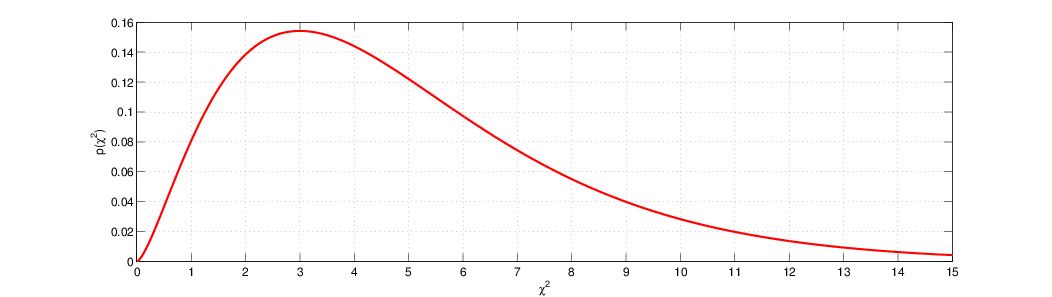
\includegraphics[width=0.8\textwidth]{chi2.png}
		\end{center}
		
		Условия применимости критерия:
		\begin{itemize}
			\item $n \geq 40;$
			\item $\frac{n_{i+}n_{+j}}{n}<5$ не более, чем в 20\% ячеек.
		\end{itemize}
	}
	
	\only<2>{
		\begin{block}{Пример} Исследуется влияние препарата на некоторое заболевание. Часть испытуемых принимает препарат, часть~--- плацебо; по окончании курса определяется, произошло ли выздоровление.
		\end{block}
		\bigskip
		
		\begin{center}
			\begin{tabular}{|c|c|c|}
				\hline
				        &Выздоровели  &Нет\\\hline
				Препарат&$850$        &$870$\\\hline
				Плацебо &$380$        &$410$\\\hline
			\end{tabular}
		\end{center}
		%    $MCC = 0.0122.$
		
		\bigskip
		
		$H_0\colon$ препарат неотличим от плацебо.
		
		$H_1\colon$ эффект препарата отличается от эффекта плацебо $\Rightarrow p = 0.5398.$
	}
\end{frame}

\begin{frame}{G-критерий}
	\begin{center}
		\begin{tabular}{rl}
			выборки:                        & $X_1^n=\left(X_{11},\ldots,X_{1n}\right), X_{1}\in\{1,\ldots,K_1\}$\\
											& $X_2^n=\left(X_{21},\ldots,X_{2n}\right), \;\; X_{2}\in\{1,\ldots,K_2\}$ \\
											& выборки связанные\\
			нулевая гипотеза:               & $H_0\colon X_1$ и $X_2$ независимы\\
			альтернатива:                   & $H_1\colon H_0$ неверна\\
			статистика:                     & $G^2\left(X_1^n, X_2^n\right) = 2 \sum\limits_{i=1}^{K_1} \sum\limits_{j=1}^{K_2} n_{ij} \ln\frac{n_{ij}n}{n_{i+}n_{+j}}$ \\
			нулевое распределение:          & $\chi^2_{\left(K_1-1\right)\left(K_2-1\right)}$\\
		\end{tabular}
		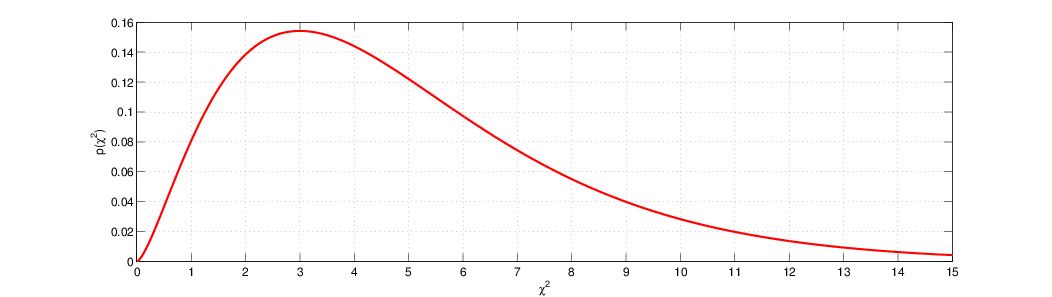
\includegraphics[width=0.8\textwidth]{chi2.png}
	\end{center}
\end{frame}

\begin{frame}{Точный критерий Фишера}
	\only<1>{
		\begin{center}
			\begin{tabular}{rl}
				выборки:                        & $X_1^{n}=\left(X_{11},\ldots,X_{1n}\right),  X_{1}\in\{0,1\}$\\
				                                & $X_2^{n}=\left(X_{21},\ldots,X_{2n}\right),  X_{2}\in\{0,1\}$\\
				                                & выборки связанные\\
				нулевая гипотеза:               & $H_0\colon X_1$ и $X_2$ независимы\\
				альтернатива:                   & $H_1\colon H_0$ неверна\\
			\end{tabular}
		\end{center}
		Пусть в таблице сопряжённости суммы по строкам и столбцам фиксированы, тогда вероятность появления наблюдаемой таблицы равна $$P\left(X_1^{n}, X_2^{n}\right) = \frac{\left(a+b\right)! \left(c+d\right)! \left(a+c\right)! \left(b+d\right)! }{a! b! c! d! n!}.$$
		Достигаемый уровень значимости определяется как сумма по всем возможным вариантам таблицы с такими же суммами по строкам и~столбцам, имеющим вероятность не более $P\left(X_1^n, X_2^n\right).$
		
		\bigskip
		
		Для односторонней альтернативы ($ad\ll bc$) достигаемый уровень значимости можно определить через гипергеометрическое распределение:
		$$p = \sum_{i=0}^a \frac{C_{a+b}^i C_{c+d}^{a+c-i}}{C_n^{a+c}}.$$
	}
	
	\only<2>{
		\begin{block}{Пример} Для 26~опрошенных известен пол и сидят ли они на диете. Есть ли связь между этими признаками?
		\end{block}
		\bigskip
		
		\begin{center}
			\begin{tabular}{|c|c|c|}
				\hline
				&М  &Ж \\\hline
				На диете    &$1$  &$9$ \\\hline
				Не на диете &$13$ &$3$ \\\hline
			\end{tabular}
		\end{center}
		%    $MCC = -0.6953.$
		
		\bigskip
		
		$H_0\colon$ связи нет.
		
		$H_1\colon$ признаки связаны.
		
		Точный критерий Фишера: $p = 0.0008.$
	}
\end{frame}

\begin{frame}{Перестановочный критерий}
	Представим выборку в виде таблицы $n\times 2$:
	\begin{center}
	{\begin{tabular}{|c|c|c|}\hline
					&М  &Ж \\\hline
		На диете    &$1$  &$9$ \\\hline
		Не на диете &$13$ &$3$ \\\hline
	\end{tabular}	$\Rightarrow$
	\begin{tabular}{|c|c|}\hline
	Строка & Столбец \\\hline
	1      & 1 \\
	1      & 2 \\
	\multicolumn{2}{|c|}{\dots} \\
	1      & 2 \\
	2      & 1 \\
	\multicolumn{2}{|c|}{\dots} \\
	2      & 1 \\
	2      & 2 \\
	2      & 2 \\
	2      & 2 \\ \hline
	\end{tabular}}
	\end{center}
	
	Используем статистику критерия хи-квадрат, но её нулевое распределение будем оценивать по $n!$ перестановок второй колонки.
		
		\bigskip
		
		$H_0\colon$ связи нет.
		
		$H_1\colon$ признаки связаны.
		
		Точный критерий Фишера: $p = 0.0008.$	
		
		Критерий хи-квадрат: $p = 0.0004.$	
		
		Перестановочный критерий со статистикой хи-квадрат: $p = 0.0014.$	
\end{frame}

\subsection{Меры взаимосвязи}
\begin{frame}{Коэффициент V Крамера}
%%%%%%%%%%%%%%%%%%%%%%%%%%%%%%%%%%%%%%%%%%%%%%%%%%%%%%%%%%%%%%%%%%%%%%%
% Коэффициент Крамера принимает значения исключительно в интервале от 0 до 1, то есть он не может быть отрицательным. 0, как и раньше, соответствует полному отсутствию взаимосвязи, а 1 — полному совпадению переменных X1 и X2 с точностью до переименования уровнеи?. Корреляция между двумя категориальными переменными не может быть отрицательнои?, поскольку уровни категориальных переменных не связаны друг с другом отношениями порядков.
%%%%%%%%%%%%%%%%%%%%%%%%%%%%%%%%%%%%%%%%%%%%%%%%%%%%%%%%%%%%%%%%%%%%%%%
	Мера взаимосвязи между двумя категориальными переменными --- коэффициент $V$ Крамера:
	$$\phi_c\left(X_1^n,X_2^n\right) = \sqrt{\frac{\chi^2\left(X_1^n,X_2^n\right)}{n\left(\min\left(K_1,K_2\right)-1\right)}}.$$
	
	$\phi_c\left(X_1^n,X_2^n\right) \in [0,1];$
    
    0 соответствует полному отсутствию взаимосвязи, 1~--- совпадению переменных.
%	
%	\bigskip
%	
%	\begin{center}
%		\includegraphics[width=0.7\textwidth]{../../2013-2/6/cram.eps}
%	\end{center}
\end{frame}

\begin{frame}{Корреляция между порядковыми переменными}
	Мера взаимосвязи между двумя порядковыми переменными --- коэффициент $\gamma$:
	$$\hat{\gamma} = \frac{p_C-p_D}{n^2-p_t},$$
	где $p_C = \frac{C}{n}$~--- частота появления согласованных пар элементов выборки, т.\,е., таких, что $i_1>i_2, \; j_1>j_2$ или $i_1<i_2, \; j_1<j_2$;
	 		
	$p_D=\frac{D}{n}$~--- частота несогласованных пар;
	
	$p_t = \frac{T}{n}$~--- частота таких пар, что $i_1=i_2$ или $j_1=j_2$.
	
	$\gamma \in [-1,1];$ $-1$ соответствует полному отсутствию согласованных пар, $1$~---~отсутствию несогласованных.
\end{frame}
\begin{frame}	
\begin{block}{Пример}
	\begin{table}[h]
		\centering
		\resizebox{\textwidth}{!}{%
			\begin{tabular}{|l|c|c|c|}
				\hline
				& \multicolumn{3}{c|}{Счастье} \\ \cline{2-4} 
				Политические взгляды & Не слишком счастлив & Вполне счастлив & Очень счастлив \\ \hline
				Либеральные & 13 & 29 & 15 \\ \hline
				Умеренные & 23 & 59 & 47 \\ \hline
				Консервативные & 14 & 67 & 54 \\ \hline
			\end{tabular}
		}
	\end{table}
\end{block}
	
	\vspace{5pt}
	
	$\chi^2 = 7.07, p = 0.1322, \phi_c = 0.0742;$	
	
	$\hat{\gamma} = 0.185, \; 95$\% доверительный интервал~--- $\left[0.032, 0.338\right].$
	
\end{frame}

\begin{frame}{Корреляция Мэтьюса}
%%%%%%%%%%%%%%%%%%%%%%%%%%%%%%%%%%%%%%%%%%%%%%%%%%%%%%%%%%%%%%%%%%%%%%%
% Коэффициент корреляции Мэтьюса — это мера силы взаимосвязи между двумя бинарными переменными. Для того чтобы его вычислить, необходимо использовать таблицу сопряженности. В строках таблицы сопряже?нности находятся значения одного признака, по столбцам — второго, в каждои? ячеи?ке — количество объектов, на которых реализовалась эта пара.
% Точно так же, как и коэффициенты Пирсона и Спирмена, корреляция Мэтьюса лежит в диапазоне от ?1 до 1. MCCX1X2 = 0 точно так же соответствует случаю полного отсутствия взаимосвязи между переменными. MCCX1X2 = 1 соответствует ситуации, когда у X1 и X2 полностью совпадают, то есть b = c = 0, в выборке отсутствуют объекты, на которых значения X1 и X2 отличаются. MCCX1X2 = ?1 — это противоположная ситуация: в выборке нет ни одного объекта, на которых значения двух бинарных признаков совпадают.
%%%%%%%%%%%%%%%%%%%%%%%%%%%%%%%%%%%%%%%%%%%%%%%%%%%%%%%%%%%%%%%%%%%%%%%
	Мера взаимосвязи между двумя бинарными переменными~--- коэффициент корреляции Мэтьюса:
	$$MCC = \frac{ad-bc}{\sqrt{(a+b)(a+c)(b+d)(c+d)}}.$$
	
	$MCC\in[-1,1];$ 0 соответствует полному отсутствию взаимосвязи, 1~---~нулям на побочной диагонали, $-1$~--- нулям на главной диагонали.
\end{frame}

	\begin{frame}{Пары переменных разных типов}
	Между категориальными и непрерывными признаками корреляции считать не нужно!
	
	\bigskip
	
	Пусть $X_1\in \mathbb{R}, X_2\in\left\{0,1\right\};$ 
	
	$X_1$ и $X_2$ положительно коррелированы, если $\mathbb{E}\left(X_1\left.\right|X_2=1\right) > \mathbb{E}\left(X_1\left.\right|X_2=0\right)$.
	
	\bigskip
	
	Мера взаимосвязи $X_1$ и $X_2$~--- разность $\mathbb{E}\left(X_1\left.\right|X_2=1\right) - \mathbb{E}\left(X_1\left.\right|X_2=0\right)$.
\end{frame}

\subsection{Парадокс хи-квадрат}
\begin{frame}{Парадокс хи-квадрат (Симпсона)}
	\only<1>{
		Эксперимент: пациенты принимают препарат или плацебо, по окончании курса определяется, выздоровели они или нет.
		
		Есть ли связь между выздоровлением и приёмом препарата?
		
		\bigskip
		
		\begin{center}
			\begin{tabular}{|c|cc|}
				\hline
				Мужчины &Выздоровели&Нет\\\hline
				Препарат&$700$        &$800$ \\
				Плацебо & $80$        &$130$ \\
				\hline
			\end{tabular}
			\quad
			\begin{tabular}{|c|cc|}
				\hline
				Женщины &Выздоровели&Нет\\\hline
				Препарат&$150$        &$70$ \\
				Плацебо &$300$       &$280$\\
				\hline
			\end{tabular}
		\end{center}
		Для мужчин: $\chi^2 = 5.456, \; p = 0.0195.$
		
		Для женщин: $\chi^2 = 17.555, \; p = 2.8 \times 10^{-5}.$
		
		\bigskip
		
		\begin{center}
			\begin{tabular}{|c|cc|}
				\hline
				М+Ж     &Выздоровели&Нет\\\hline
				Препарат&$850$        &$870$ \\
				Плацебо &$380$        &$410$\\
				\hline
			\end{tabular}
		\end{center}
		Суммарно: $\chi^2 = 0.376, \; p = 0.5398.$
	}
	
	\only<2>{
		Причины несогласованности выводов~--- большие отличия в размерах групп пациентов, принимающих плацебо и препарат: основной вклад в~выводы вносят женщины, принимавшие плацебо, и мужчины, принимавшие препарат.
		
		\bigskip
		
		Чтобы такого не происходило, плацебо и препарат должны поровну распределяться по всем анализируемым подгруппам.
	}
\end{frame}

\begin{frame}{Парадокс хи-квадрат (Симпсона)}
	\only<1>{
		\begin{block}{Пример, Bikel at el., 1975} В~1973 году на университет Беркли, Калифорния, подали в суд: доля поступивших абитуриентов мужского пола была выше, чем доля поступивших женского пола.
        \end{block}
		
		\begin{center}
			\begin{tabular}{|c|cc|c|}
				\hline
				& Не поступили&Поступили&Доля поступивших\\\hline
				Мужчины & $4704$        &$3738$     & $44.3\%$\\
				Женщины & $2827$        &$1494$     & $34.6\%$\\      \hline
			\end{tabular}
		\end{center}
%		
%		\bigskip
%		
%		\begin{center}
%			\includegraphics[width=0.3\textwidth]{../../2013-2/6/woman.eps}
%		\end{center}
	}
	
	\only<2>{
		Критерий хи-квадрат: $\chi^2 = 108.1, \; p \approx 0.$
		
		\bigskip
		
		\begin{center}
		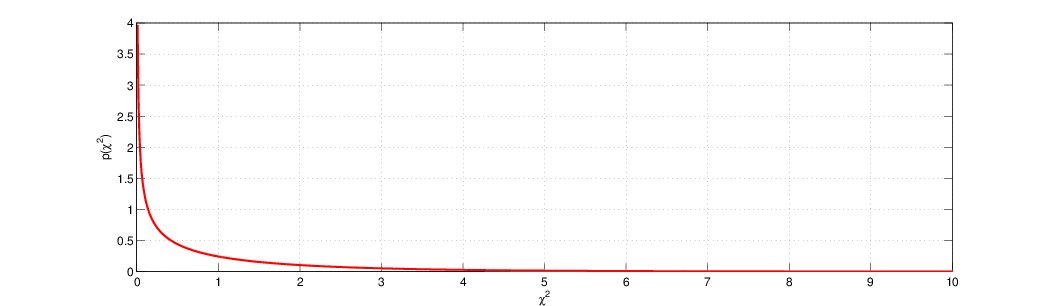
\includegraphics[width=0.8\textwidth]{chi21.png}
		\end{center}
		
		\bigskip
		
		\begin{center}
			\begin{tabular}{|c|cc|cc|cc|}
				\hline
				&\multicolumn{2}{c|}{Наблюдаемые} & \multicolumn{2}{c|}{Ожидаемые} & \multicolumn{2}{c|}{Разности} \\
				& -           &+                   & -                & +            & -                   & +        \\\hline
				Мужчины & $4704$      &$3738$              & $4981.3$         & $3460.7$     & $-227.3$            & $227.3$  \\
				Женщины & $2827$      &$1494$              & $2549.7$         & $1771.3$     & $227.3$             & $-227.3$ \\\hline
			\end{tabular}
		\end{center}
	}
	
	\only<3>{
		Будем искать виноватых: посмотрим детализированную статистику по~85~факультетам.
		
		\bigskip
		
		Значимо (при $\alpha=0.05$) меньше женщин прошли отбор на 4 факультета, суммарный дефицит по ним --- 26.
		
		На 6 факультетов поступило значимо меньше мужчин, суммарный дефицит --- 64.
		
		\bigskip
		
		Данные по 6 крупнейшим факультетам:
		\begin{center}
			\begin{tabular}{|c|cc|cc|}
				\hline
				&\multicolumn{2}{c|}{Мужчины} & \multicolumn{2}{c|}{Женщины} \\
				& $\sum$      & +              & $\sum$        & +             \\\hline
				$1$       & $825$         & $62\%$           & $108$           & $\boldsymbol{82\%}$ \\
				$2$       & $560$         & $63\%$           & $25$            & $\boldsymbol{68\%}$ \\
				$3$       & $325$         & $\boldsymbol{37\%}$  & $593$           & $34\%$          \\
				$4$       & $417$         & $33\%$           & $375$           & $\boldsymbol{35\%}$ \\
				$5$       & $191$         & $\boldsymbol{28\%}$  & $393$           & $24\%$          \\
				$6$       & $272$         & $6\%$            & $341$           & $\boldsymbol{7\%}$  \\\hline
			\end{tabular}
		\end{center}
		
	}
	
	\only<4>{
		Ответ: женщины чаще пытались поступить на факультеты с большим конкурсом.
		\begin{center}
			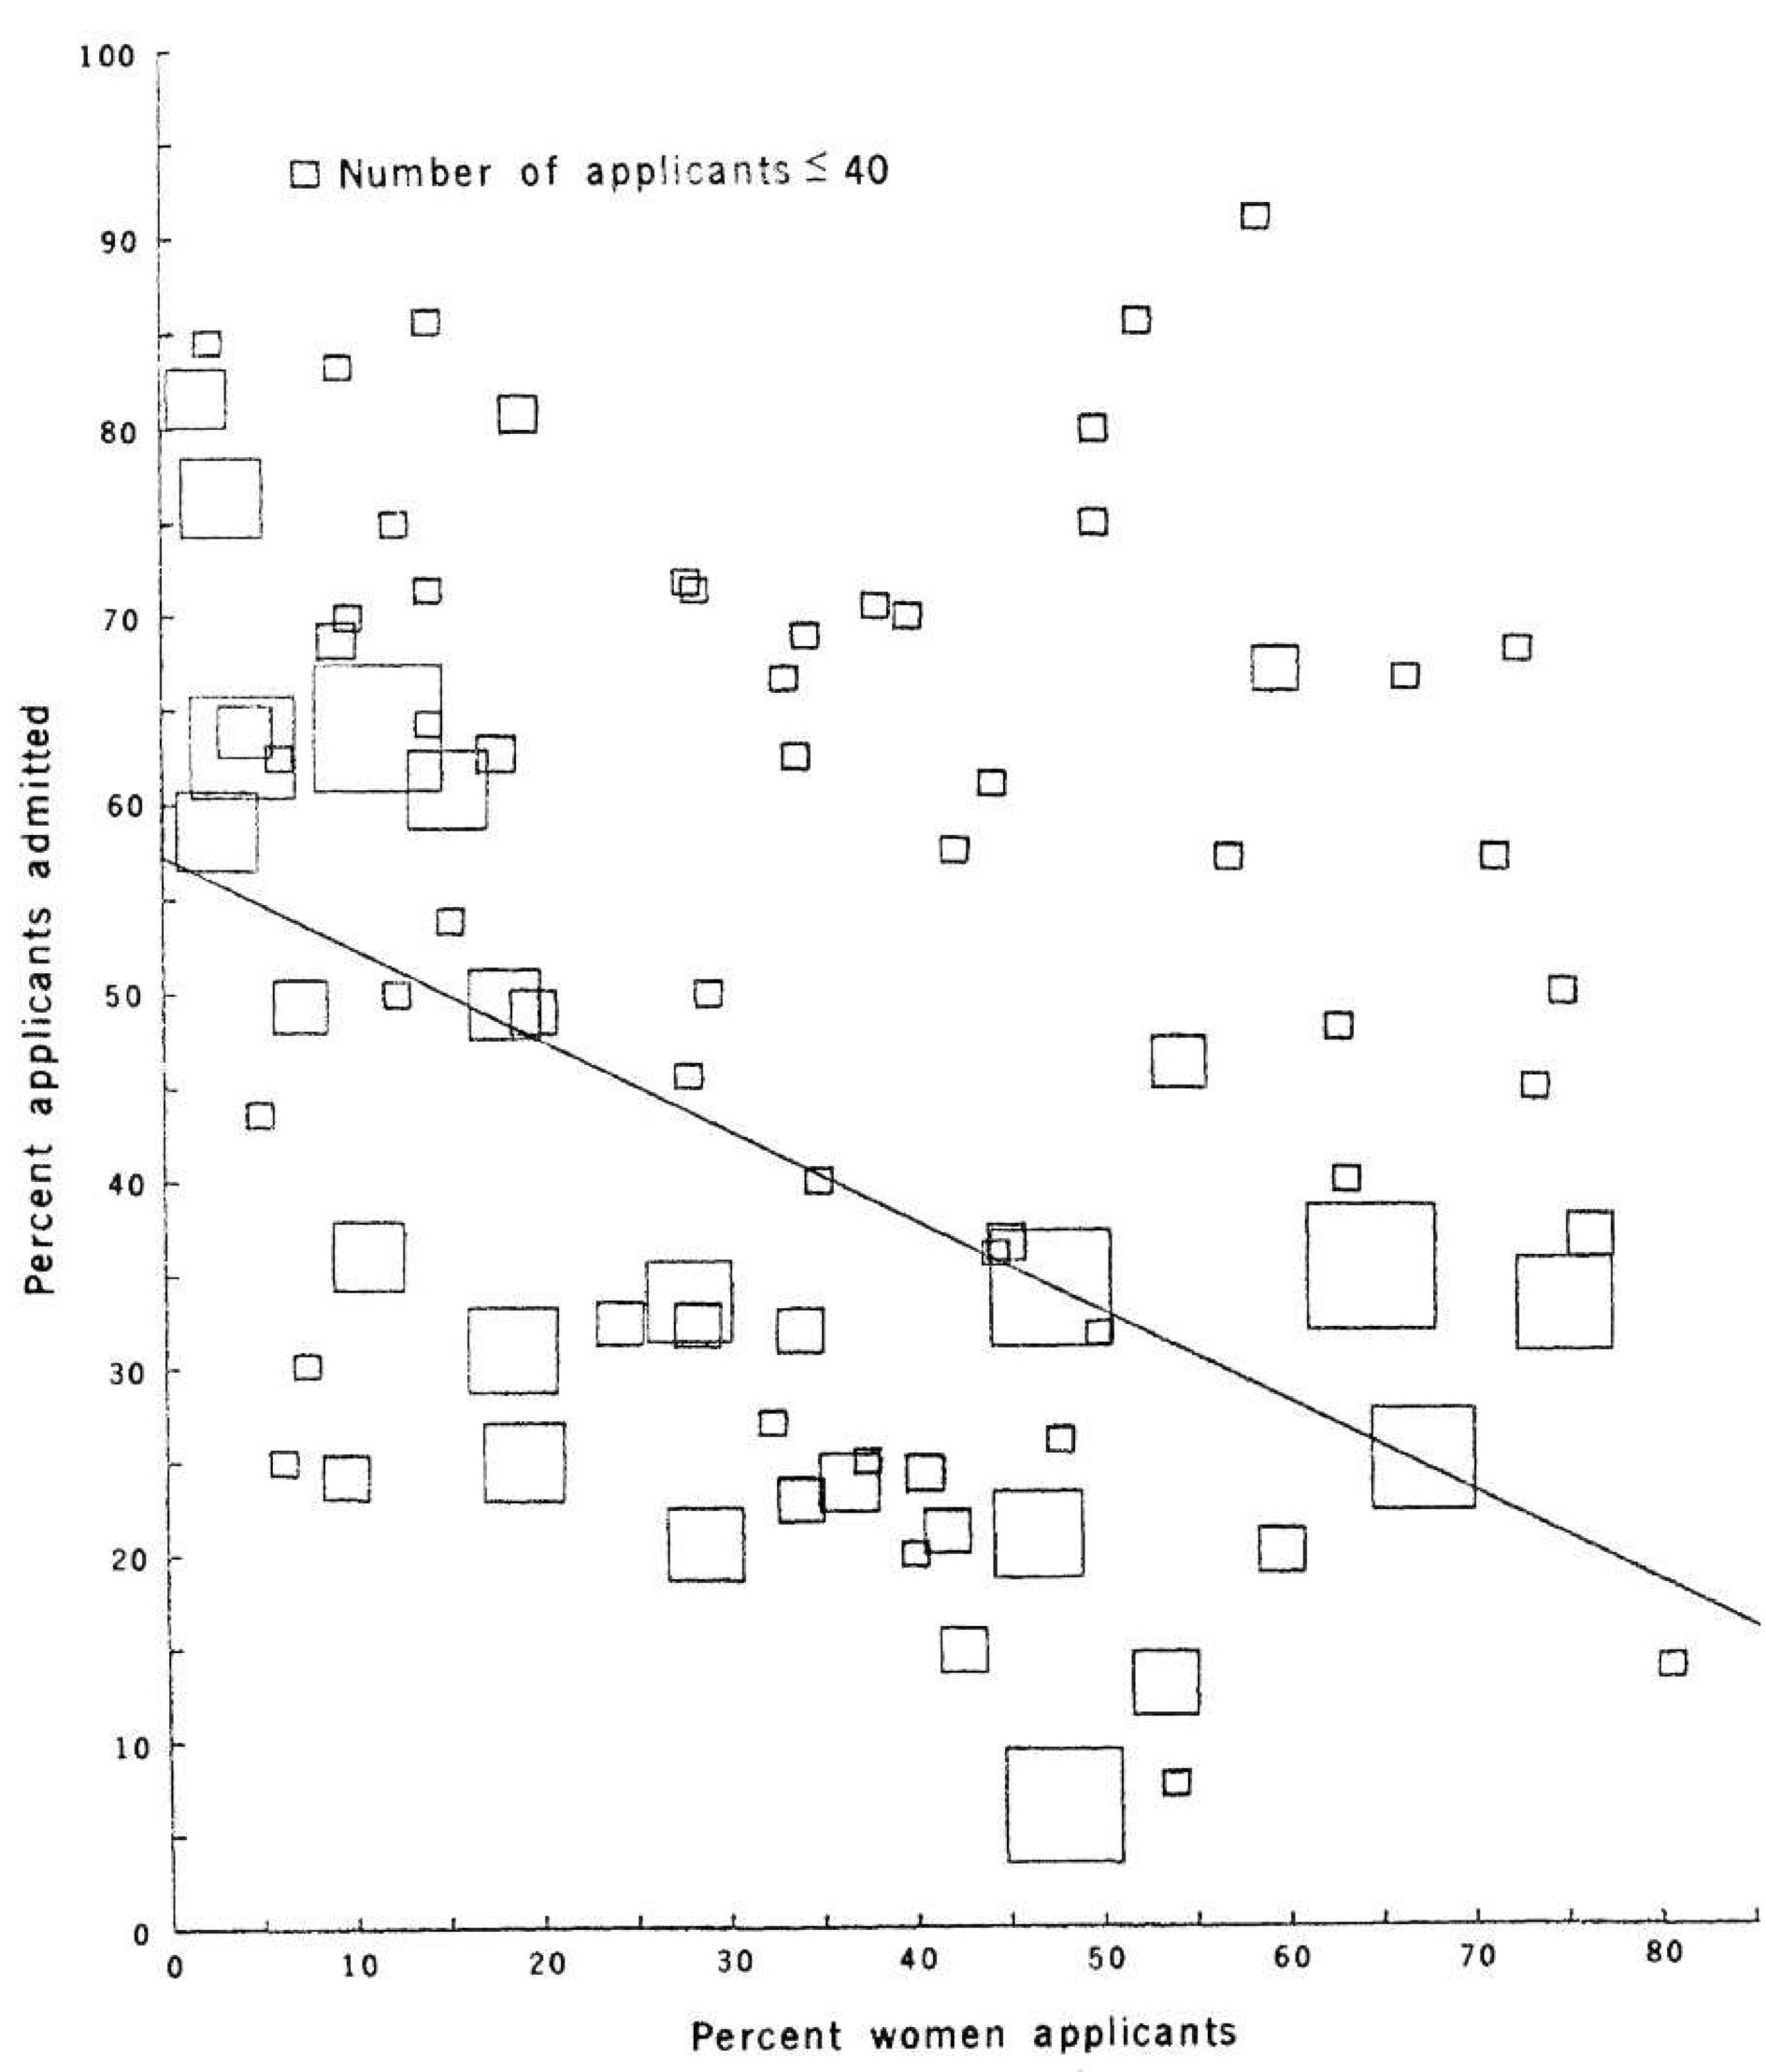
\includegraphics[height=0.8\textheight]{berkeley.png}
		\end{center}
	}
	
	\only<5>{
	“Like fire, the chi-square statistic is an excellent servant and a bad master.” (Austin Bradford Hill)}
\end{frame}

\section{}
\begin{frame}{Литература}
	\begin{itemize}
		\item непрерывные признаки~--- Лагутин, гл.\,20;
		\item категориальные признаки~--- Agresti, гл.\,2 и 3, Bilder, разделы 3.1, 3.2, 6.2.1, 6.2.2;
		\item значимость корреляции Пирсона~--- Kanji, №12, Good, 3.8;
		\item значимость корреляции Кендалла и Спирмена~--- Кобзарь, 5.2.2.2.1, 5.2.2.2.2;
		\item значимость частной и множественной корреляций~--- Кобзарь, 5.2.1.3.
%		\item канонические корреляции~--- Tabachnick, гл.\,12.
	\end{itemize}
	
	\bigskip
	
	{\small
		Кобзарь А.И. \textit{Прикладная математическая статистика}, 2006.
		
		\vspace{5pt}
		    	
		Лагутин М.Б. \textit{Наглядная математическая статистика}, 2007.
		
		\vspace{5pt}
		    	
		Agresti A. \textit{Categorical Data Analysis}, 2013.
		
		\vspace{5pt}
		    	
		Bickel P.J., Hammel E.A., O’connell J.W. (1975). \textit{Sex bias in graduate admissions: data from Berkeley}. Science, 187(4175), 398–404. 
		
		\vspace{5pt}
		    			
		Bilder C.R., Loughin T.M. \textit{Analysis of Categorical Data with R}, 2013.
		
		\vspace{5pt}
		    	
		Good P. \textit{Permutation, Parametric and Bootstrap Tests of Hypotheses: A Practical Guide to Resampling Methods for Testing Hypotheses}, 2005.
		
		\vspace{5pt}
		    	
		Kanji G.K. \textit{100 statistical tests}, 2006.
%		
%		\vspace{5pt}
%		    	
%   		Tabachnick B.G., Fidell L.S. \textit{Using Multivariate Statistics}. — Boston: Pearson Education, 2012.

	}
\end{frame}

\end{document}
